\documentclass{beamer}
%\usetheme{Copenhagen}
%\usetheme{Boadilla}
\usepackage{geometry}                % See geometry.pdf to learn the layout options. There are lots.
\usepackage{graphicx}
\usepackage{amssymb}
\usepackage{beamerthemeshadow}
 \usepackage{feynmp}
 \usepackage{textpos}
 \usepackage{biblatex}
 \usepackage{bbold}

  \usepackage{ulem}
  \usepackage{amsmath,amssymb} 
 \bibliography{foo}
  \DeclareGraphicsRule{*}{mps}{*}{} 
  % figures
  
 % \logo{
\includegraphics[height=1.2cm]{lhcblogo.jpg}\vspace{220pt}}
  
  
\usepackage{caption}
\usepackage{subfig}
\newcommand{\Lagr}{\mathcal{L}}
\setbeamertemplate{itemize item}{\scriptsize\raise1.25pt\hbox{\donotcoloroutermaths$\blacktriangleright$}}
\setbeamertemplate{itemize subitem}{\tiny\raise1.5pt\hbox{\donotcoloroutermaths$\square$}}
\setbeamertemplate{itemize subsubitem}{\tiny\raise1.5pt\hbox{\donotcoloroutermaths$\blacktriangleright$}}
\setbeamertemplate{enumerate item}{\insertenumlabel.}
\setbeamertemplate{enumerate subitem}{\insertenumlabel.\insertsubenumlabel}
\setbeamertemplate{enumerate subsubitem}{\insertenumlabel.\insertsubenumlabel.\insertsubsubenumlabel}
\setbeamertemplate{enumerate mini template}{\insertenumlabel}
\begin{document}
{


\title[ Update on search for $\Lambda_{b} \rightarrow p \mu \nu$ \hspace{2em}\insertframenumber/
\inserttotalframenumber]{Update on search for $\Lambda_{b} \rightarrow p \mu \nu$}
\author[William Sutcliffe]{
\includegraphics[height=1cm,width=1.5cm]{lhcblogo.jpg} \\ William Sutcliffe, Ulrik Egede \\ \vspace{0.5cm} Imperial College London}



\date{\today}


 \frame{\titlepage

} 

\addtobeamertemplate{frametitle}{}{%
\begin{textblock*}{100mm}(.85\textwidth,-1cm)

\includegraphics[height=1cm,width=1.5cm]{lhcblogo.jpg}
\end{textblock*}}

 %%%%slide 1

% \frame{\frametitle{Outline} 
%\begin{enumerate}
%\setlength{\itemsep}{10pt}
%\item Background and motivation.
%\item Previous measurements.
%\item $V_{ub}$ with LHCb
%\item Initial generator level study
%\end{enumerate}
%}




\frame{\frametitle{Table of contents}\tableofcontents} 

\section{Context and Motivation}
 \frame{
 \frametitle{Current Status of $|V_{ub}|$}
 \begin{itemize}
  \item \normalsize{Semi-Leptonic B Decays:}
   \end{itemize}
   \hspace{1.cm} \footnotesize{Inclusive ($\bar{B} \rightarrow X_{u} l \bar{\nu}_{l}$)} \hspace{1cm}  \footnotesize{Exclusive ($\bar{B}_{0} \rightarrow \pi^{+} l \bar{\nu}_{l}$)}
    \begin{center} 
    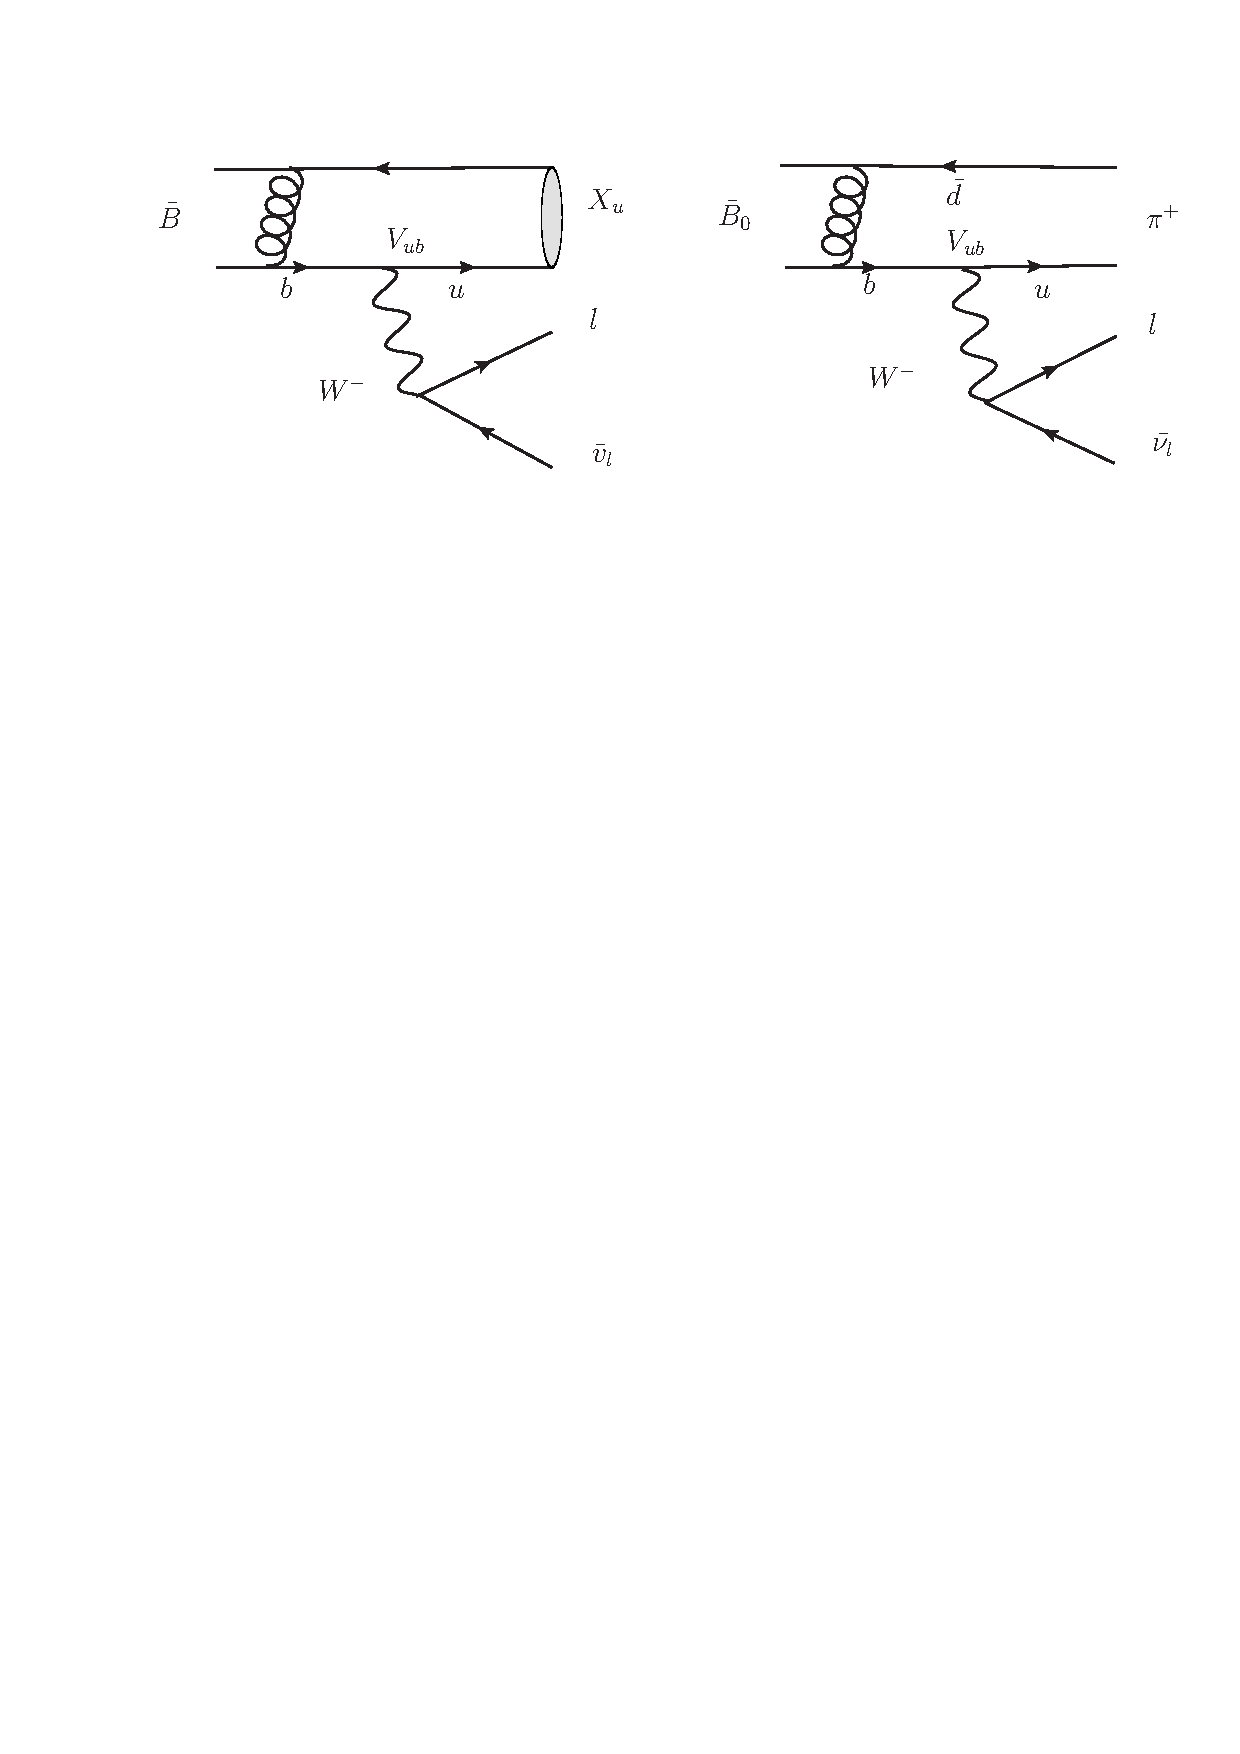
\includegraphics[trim = 15mm 215mm 0mm 25mm, clip, width=8cm]{incl_ex_feyn.pdf} 
        \end{center}
        \hspace{1.cm} \footnotesize{$|V_{ub}| = (4.41 \pm 0.15 ^{+ 0.15} _{-0.17}) \times 10^{-3}$} \hspace{0.3cm} \footnotesize{$|V_{ub}| = (3.23 \pm 0.31) \times 10^{-3}$}
  
  \vspace{0.1cm}
       \begin{itemize}
  \item \normalsize{Leptonic B decays ($B^{+} \rightarrow \tau^{+} \nu_{\tau}$):}
      \begin{center}
       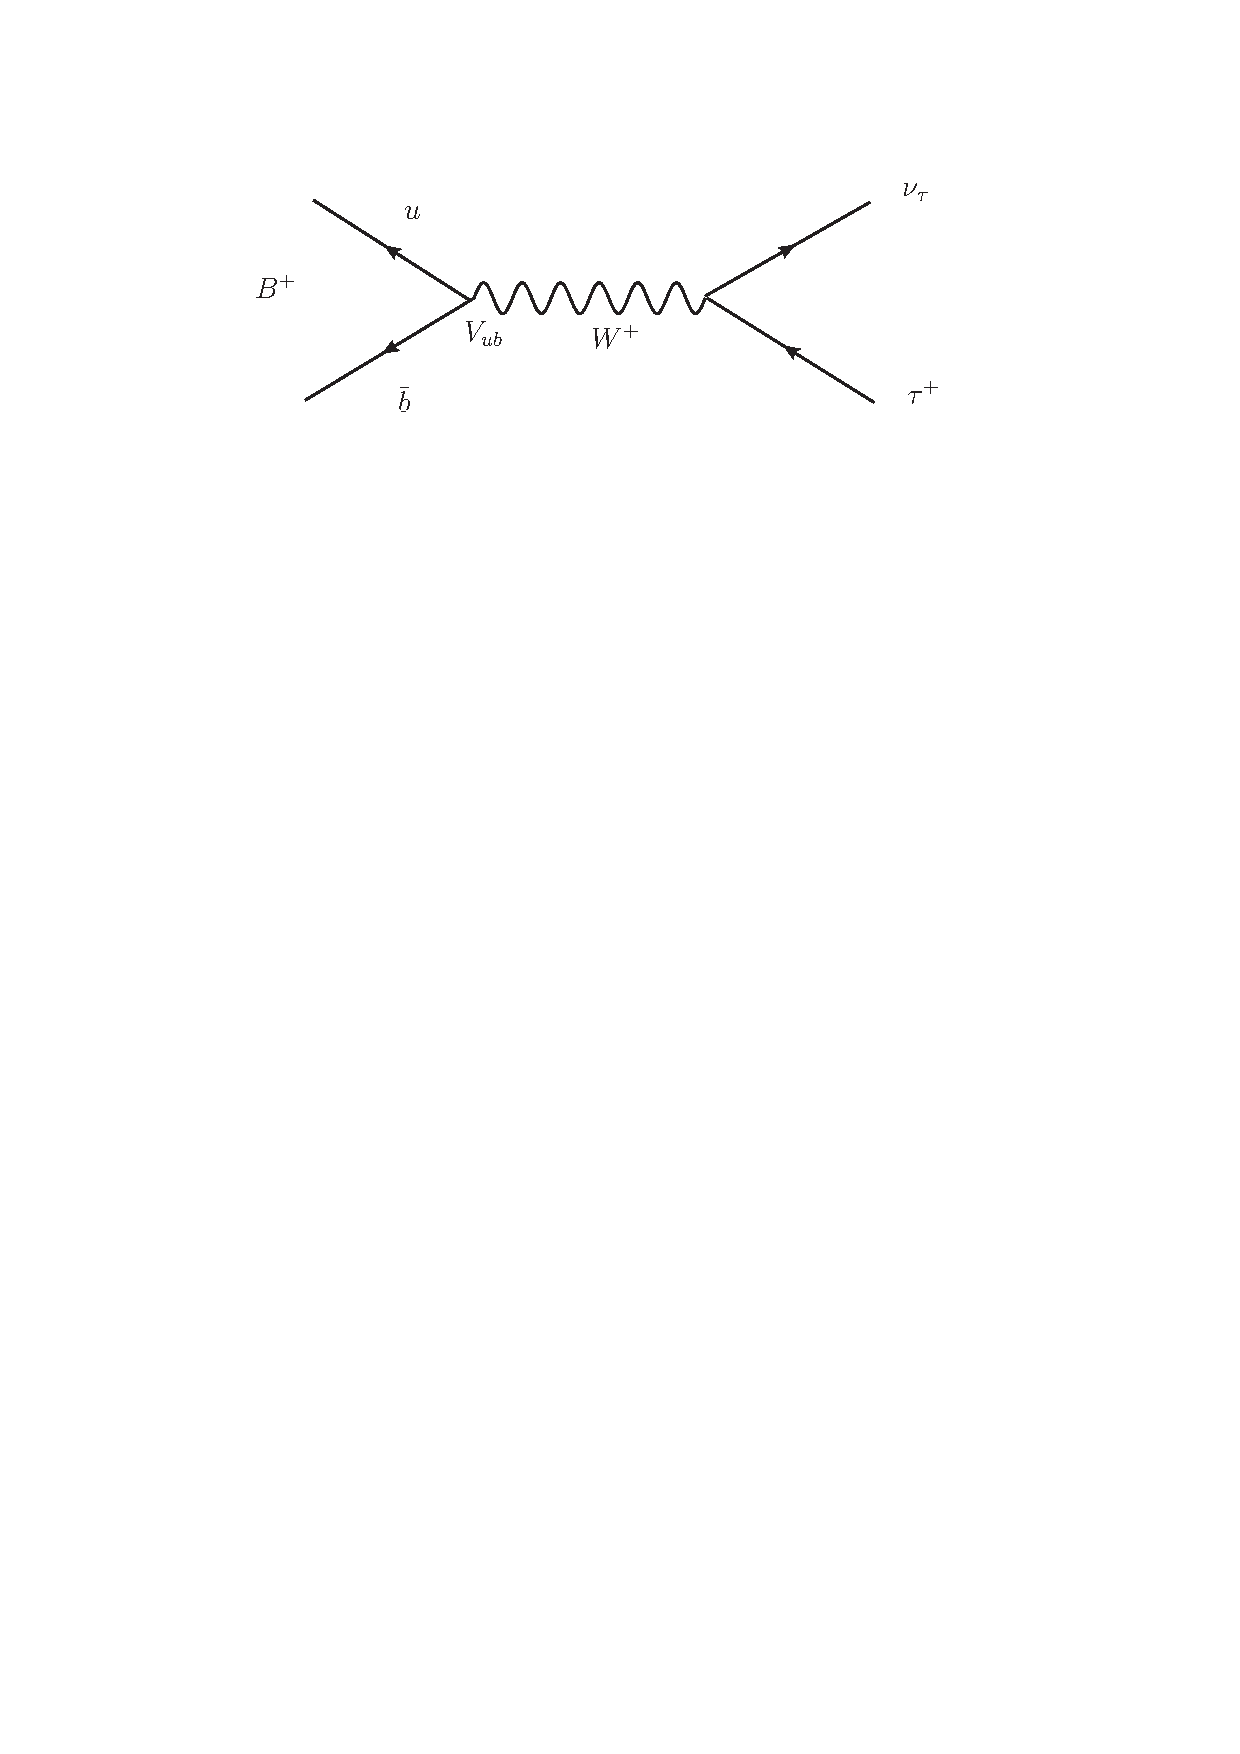
\includegraphics[trim = 15mm 215mm 0mm 30mm, clip, width=6cm]{lepfeyn.pdf} 
       \end{center}
   \end{itemize}
  

}




 \frame{
 \frametitle{$|V_{ub}|$ Constraints on the Unitarity Triangle} 
    \begin{center}
      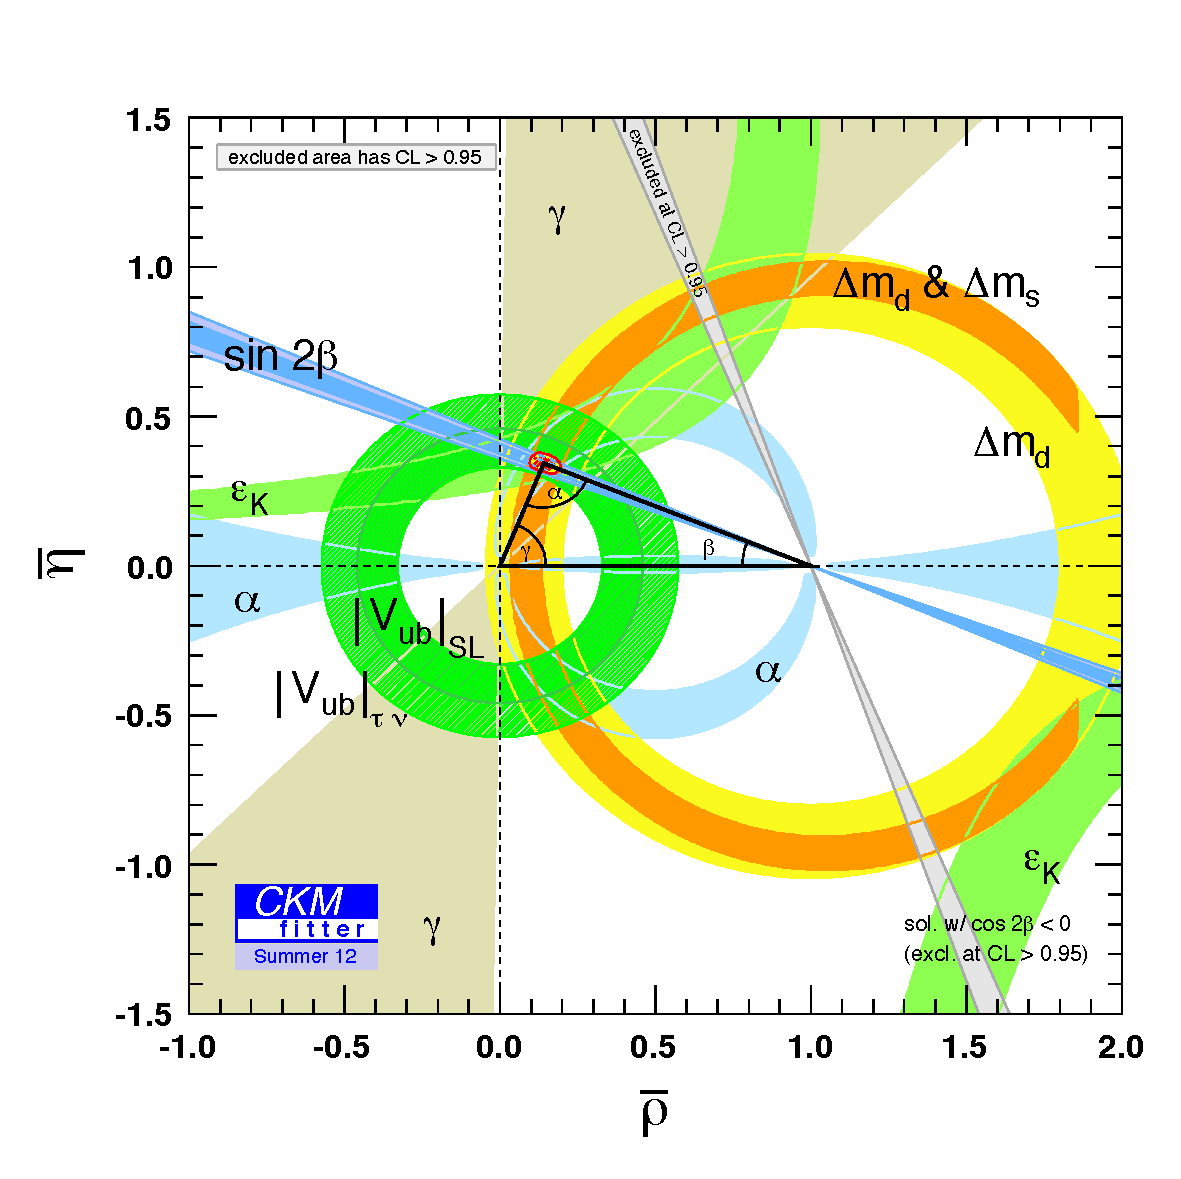
\includegraphics[width=0.6\textwidth]{CKMfit.pdf} 
        \vspace{0.0cm}
   %\hspace{1cm}\tiny{[1] CKMfitter Group, J. Charles et al. ICHEP conference (July 2012)}
  \end{center}
}

\section{Neutrino Reconstruction}
\frame{
\frametitle{Neutrino Reconstruction}
\begin{center}
      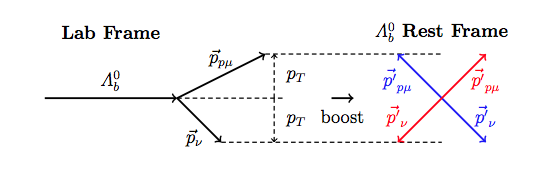
\includegraphics[width=0.6\textwidth]{nureco.png} 
\end{center}
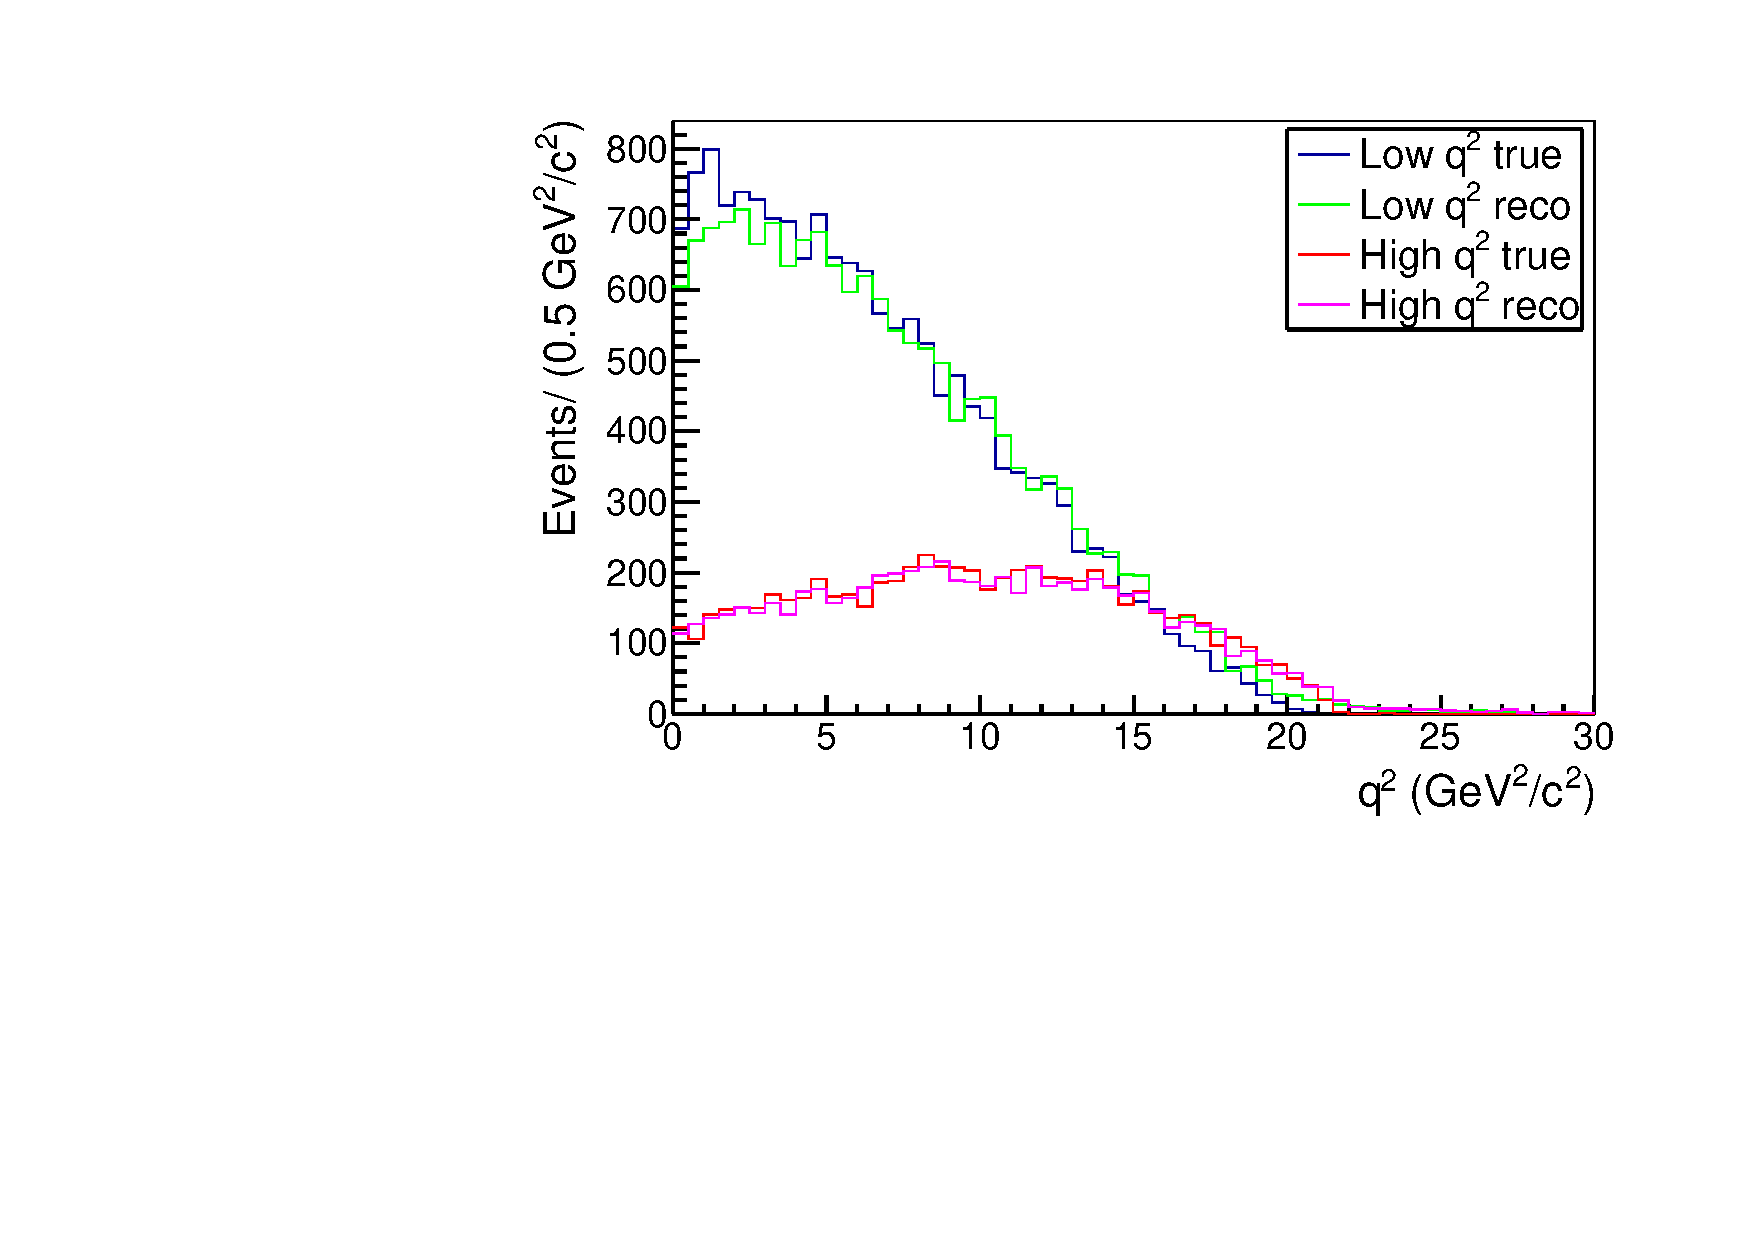
\includegraphics[width=0.5\textwidth]{q2_reco.pdf} 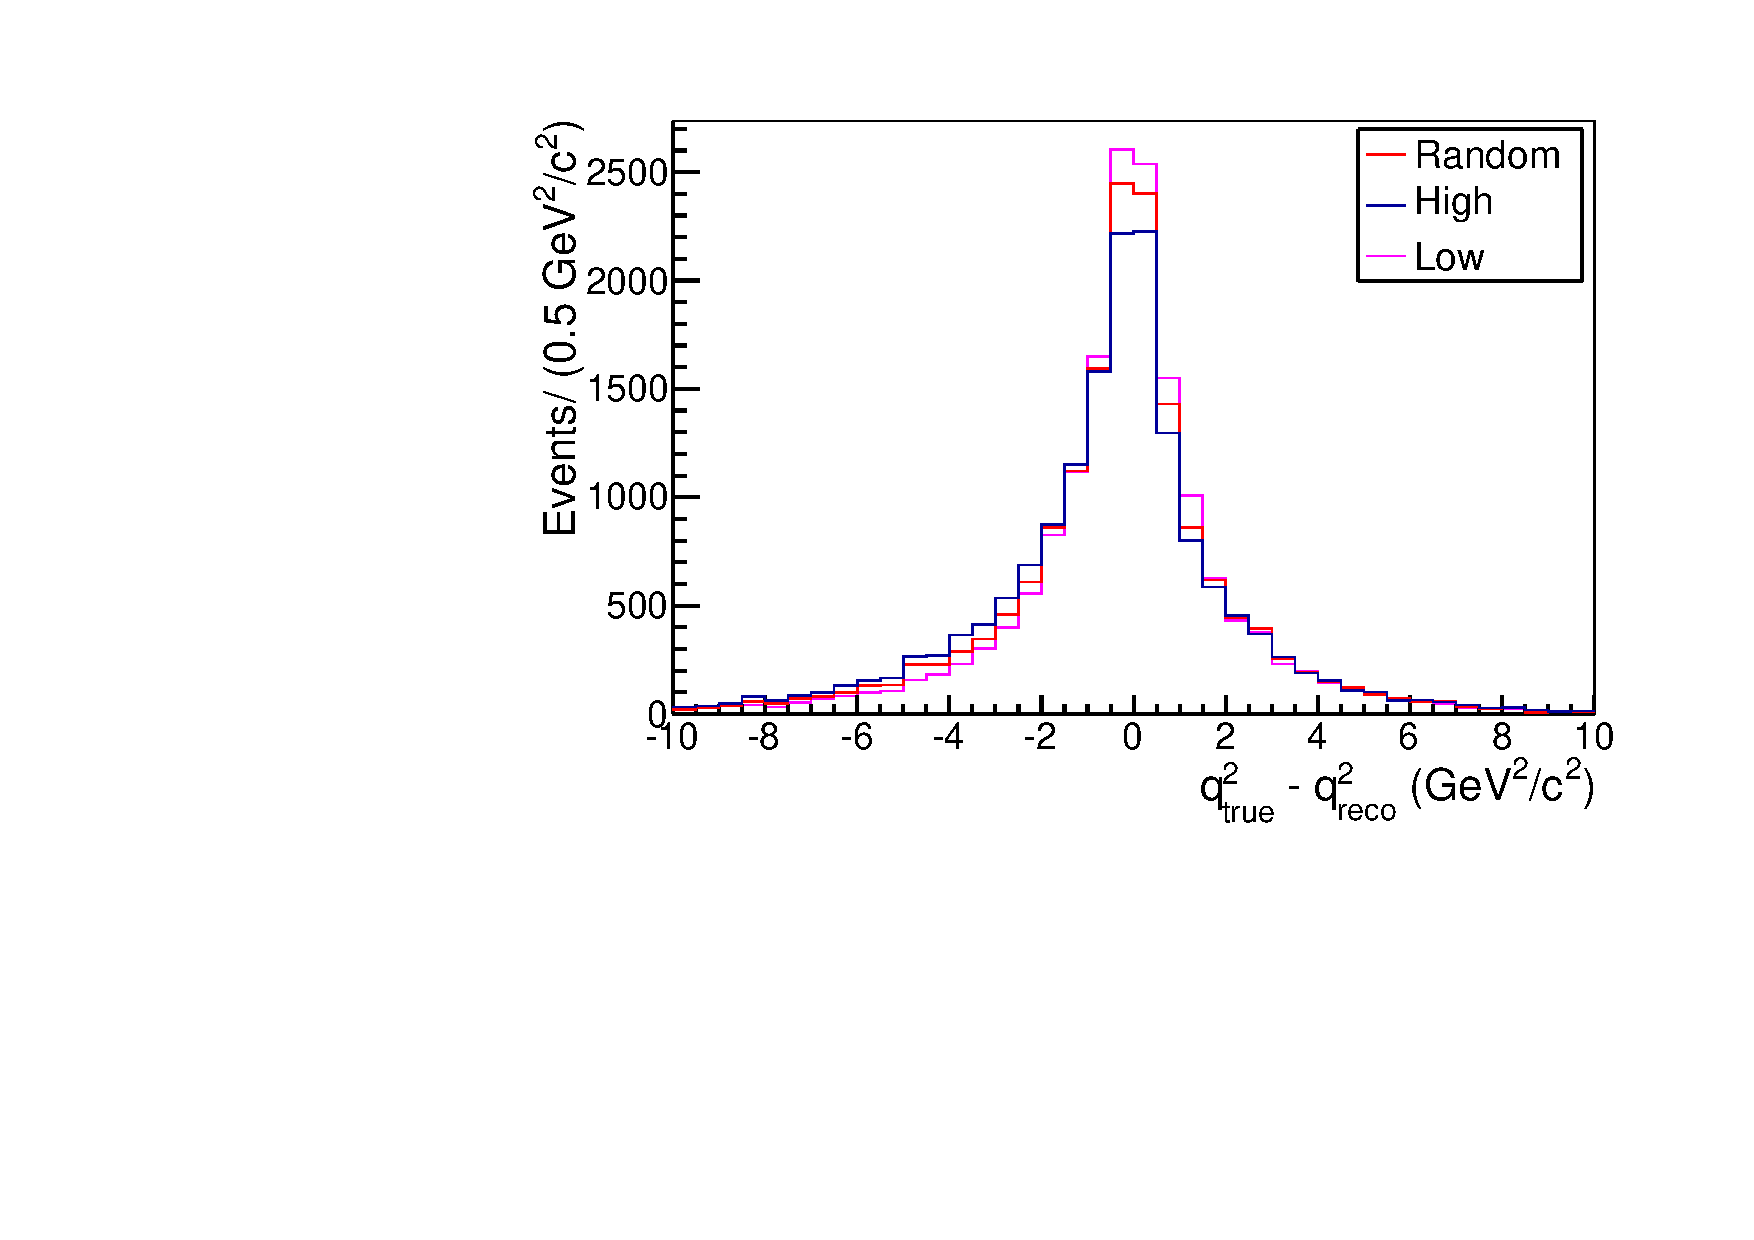
\includegraphics[width=0.5\textwidth]{qdiff.pdf} 
}


      


 
\section{Generator Level Studies}
 \frame{
 \frametitle{Generator Level Studies}
 
\begin{itemize}
 \setlength{\itemsep}{5pt}
\item Generator Level (GL) Sample of 3 million inclusive $b\overline{b}$ events.
\item Generator Level Cuts: 
\begin{itemize}
\item Within LHCb acceptance
\item At least one lepton with $p_{\rm{T}}> 1.5$ GeV/c
\end{itemize}
\item Expect this number of events in $\sim$$0.01$pb$^{-1}$ at $\sqrt{s} = 7$ TeV.
\item Search events for protons and muons produced from the decay of the same $B$ hadron.  Ignore protons and muons produced by long-lived intermediaries.
\end{itemize}
    \begin{center}
      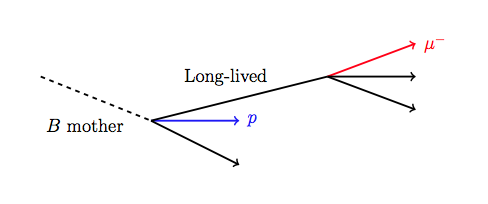
\includegraphics[width=0.5\textwidth]{GL1.png} 
   
   %\hspace{1cm}\tiny{[1] CKMfitter Group, J. Charles et al. ICHEP conference (July 2012)}
  \end{center}

}


\frame{
 \frametitle{Opposite Sign $q^{2}$ Distribution}

  \begin{center}
 \small
\begin{itemize}
  \item Plot opposite sign and same sign $p\mu$ combinations.
  \item Always choose $p$, $\overline{p}$, $\mu^{+}$, $\mu^{-}$  with highest momentum.
  \item Include normalised sample $\Lambda_{b} \rightarrow p \mu \nu$ phase space GL MC.
 
\end{itemize}
      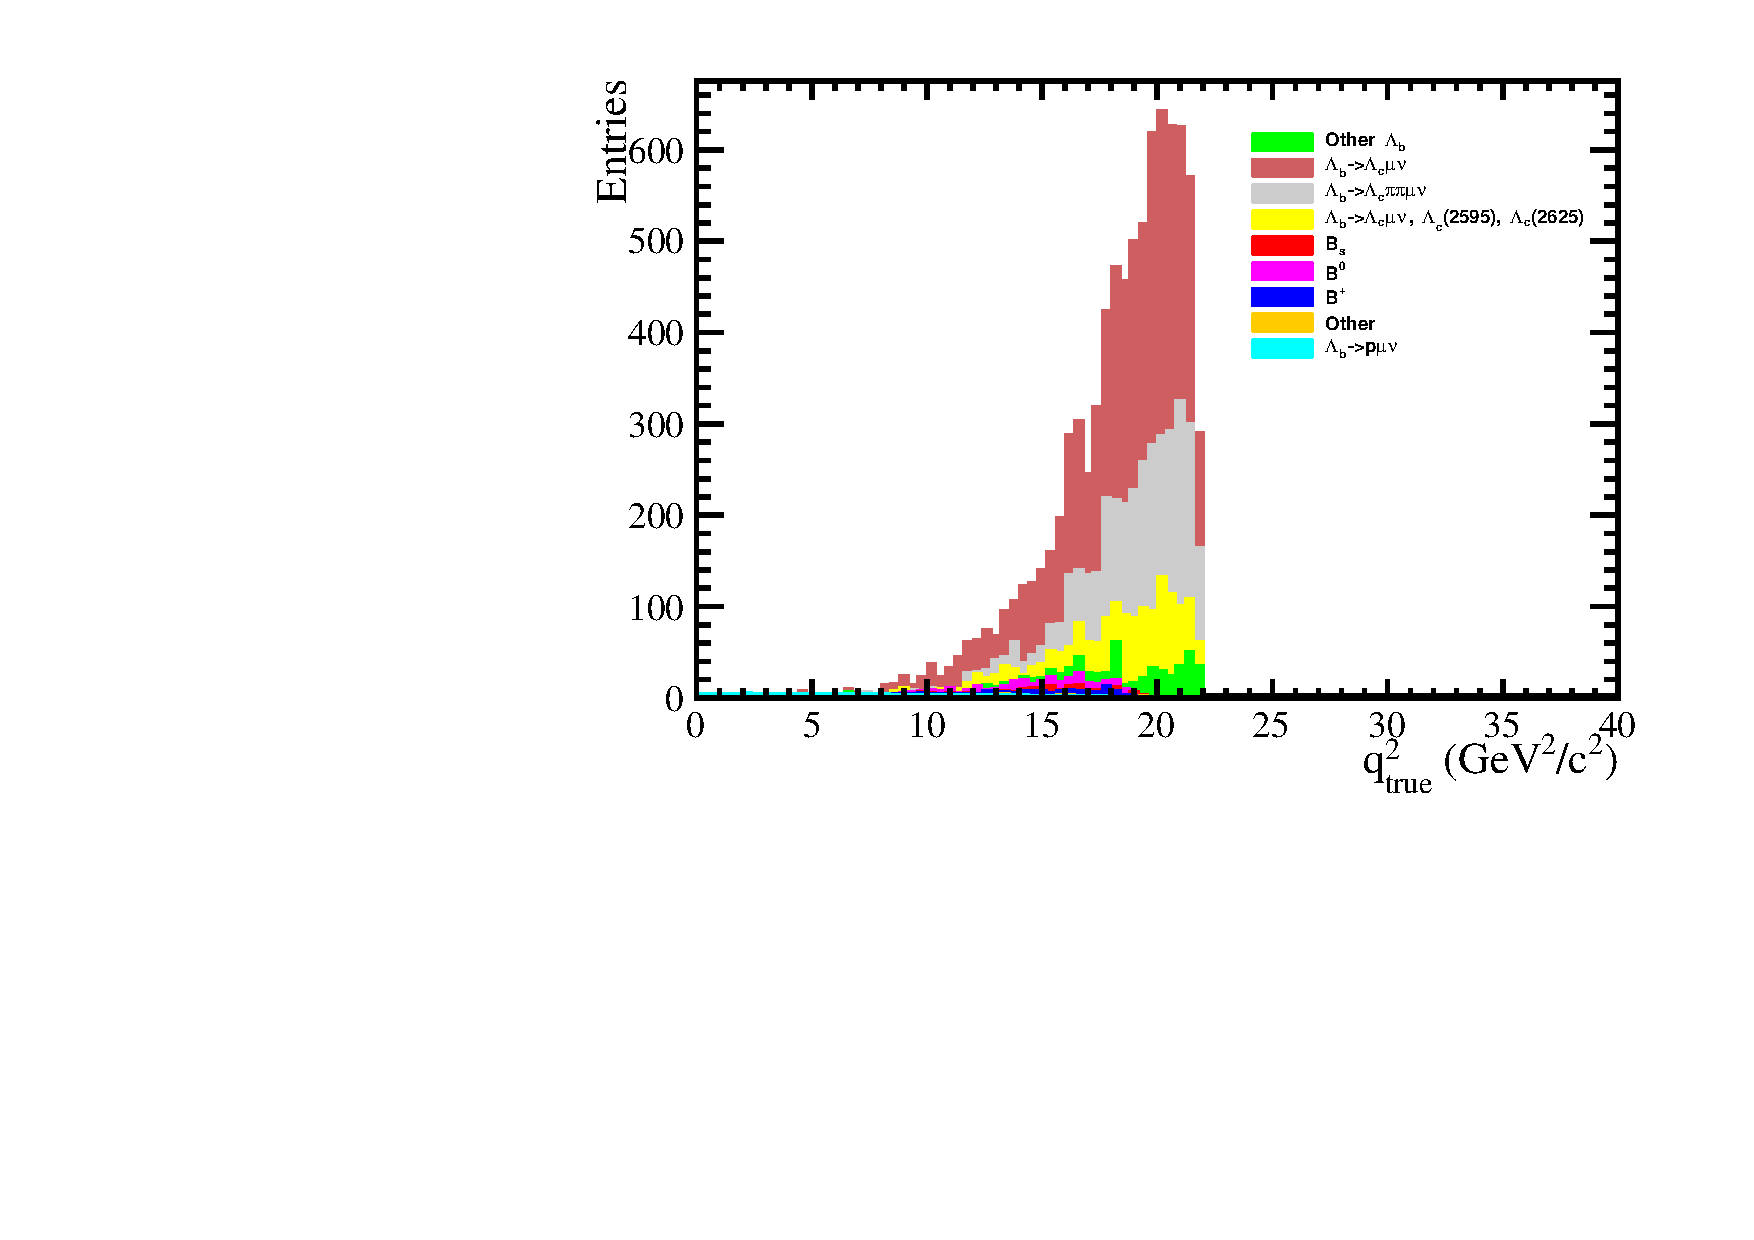
\includegraphics[width=0.7\textwidth]{q2_true_nolog.pdf} 
\end{center}
}

 \frame{
 \frametitle{Opposite Sign $p\mu$ Combinatons}


      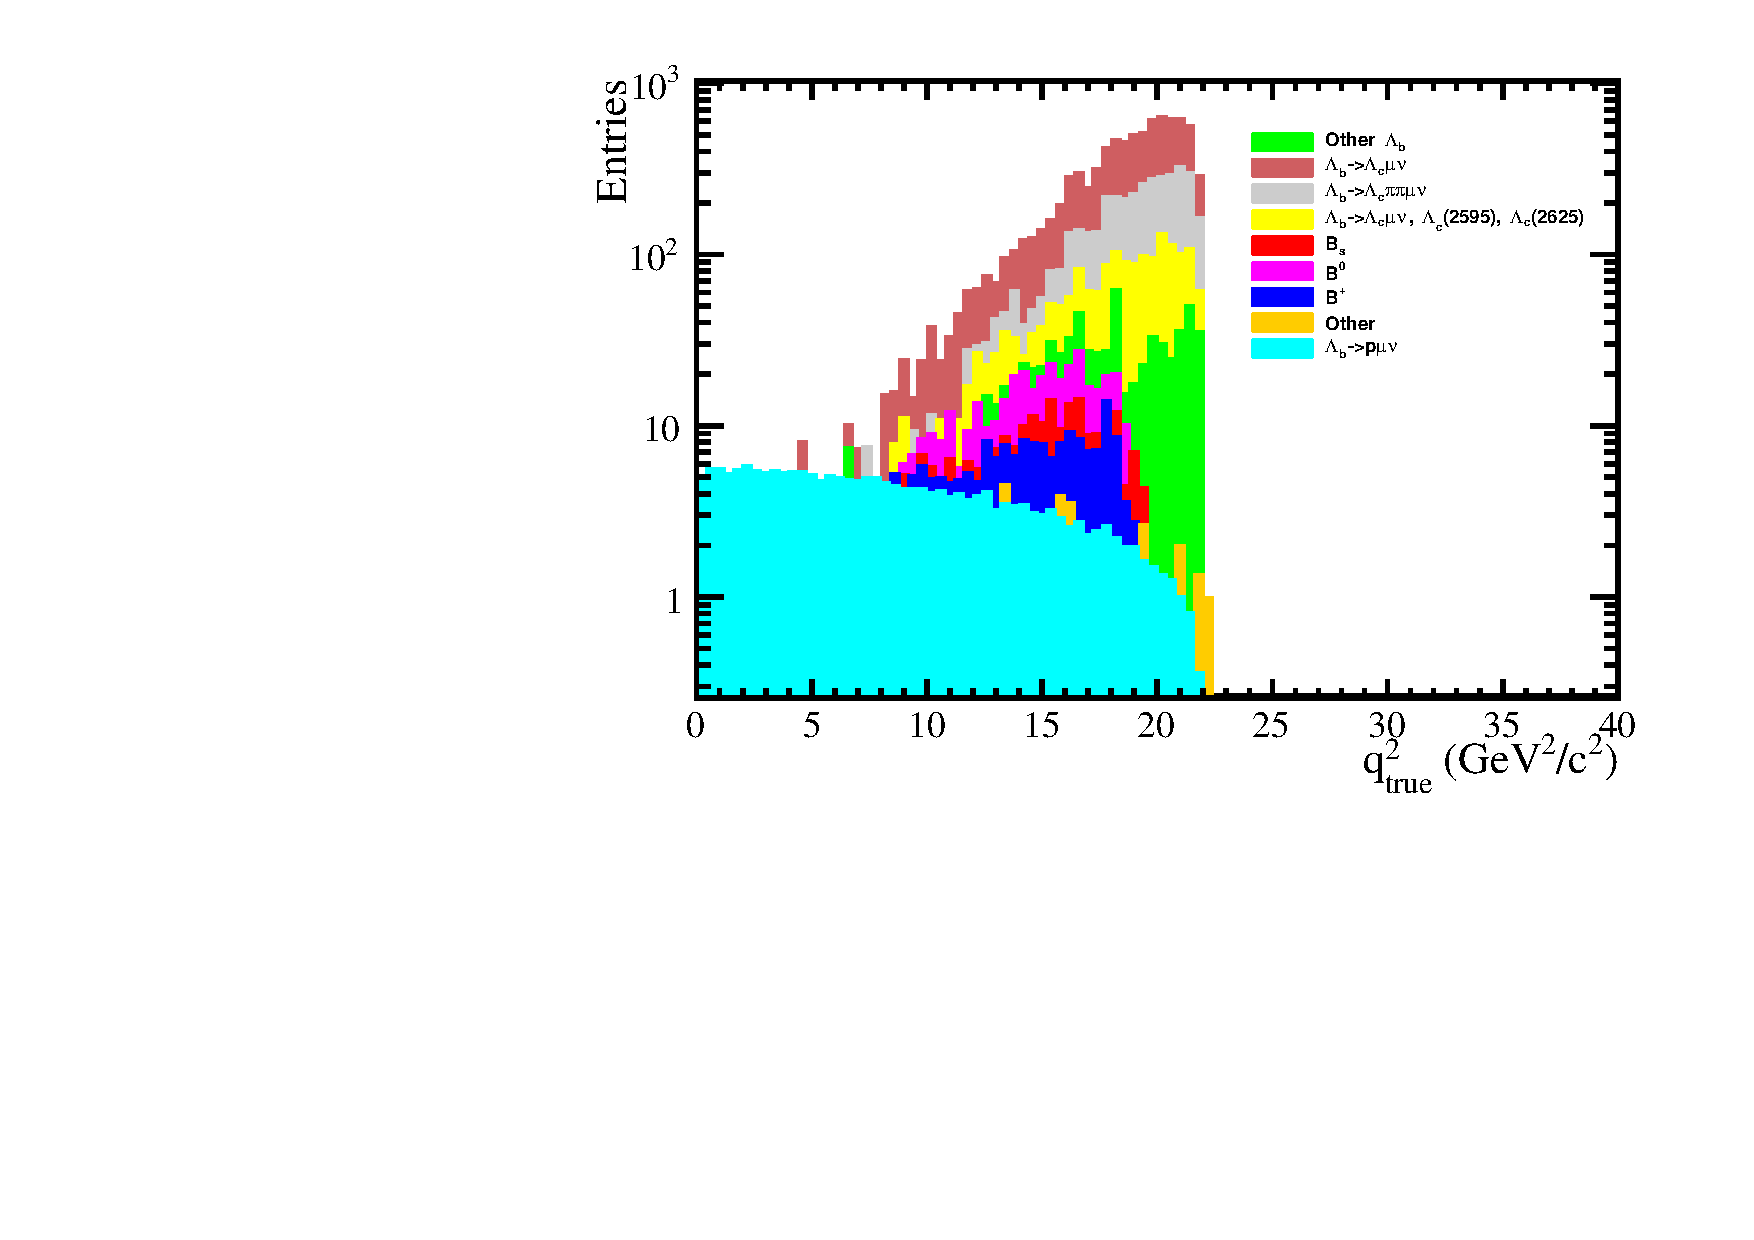
\includegraphics[width=0.45\textwidth]{q2_true_stacked.pdf}    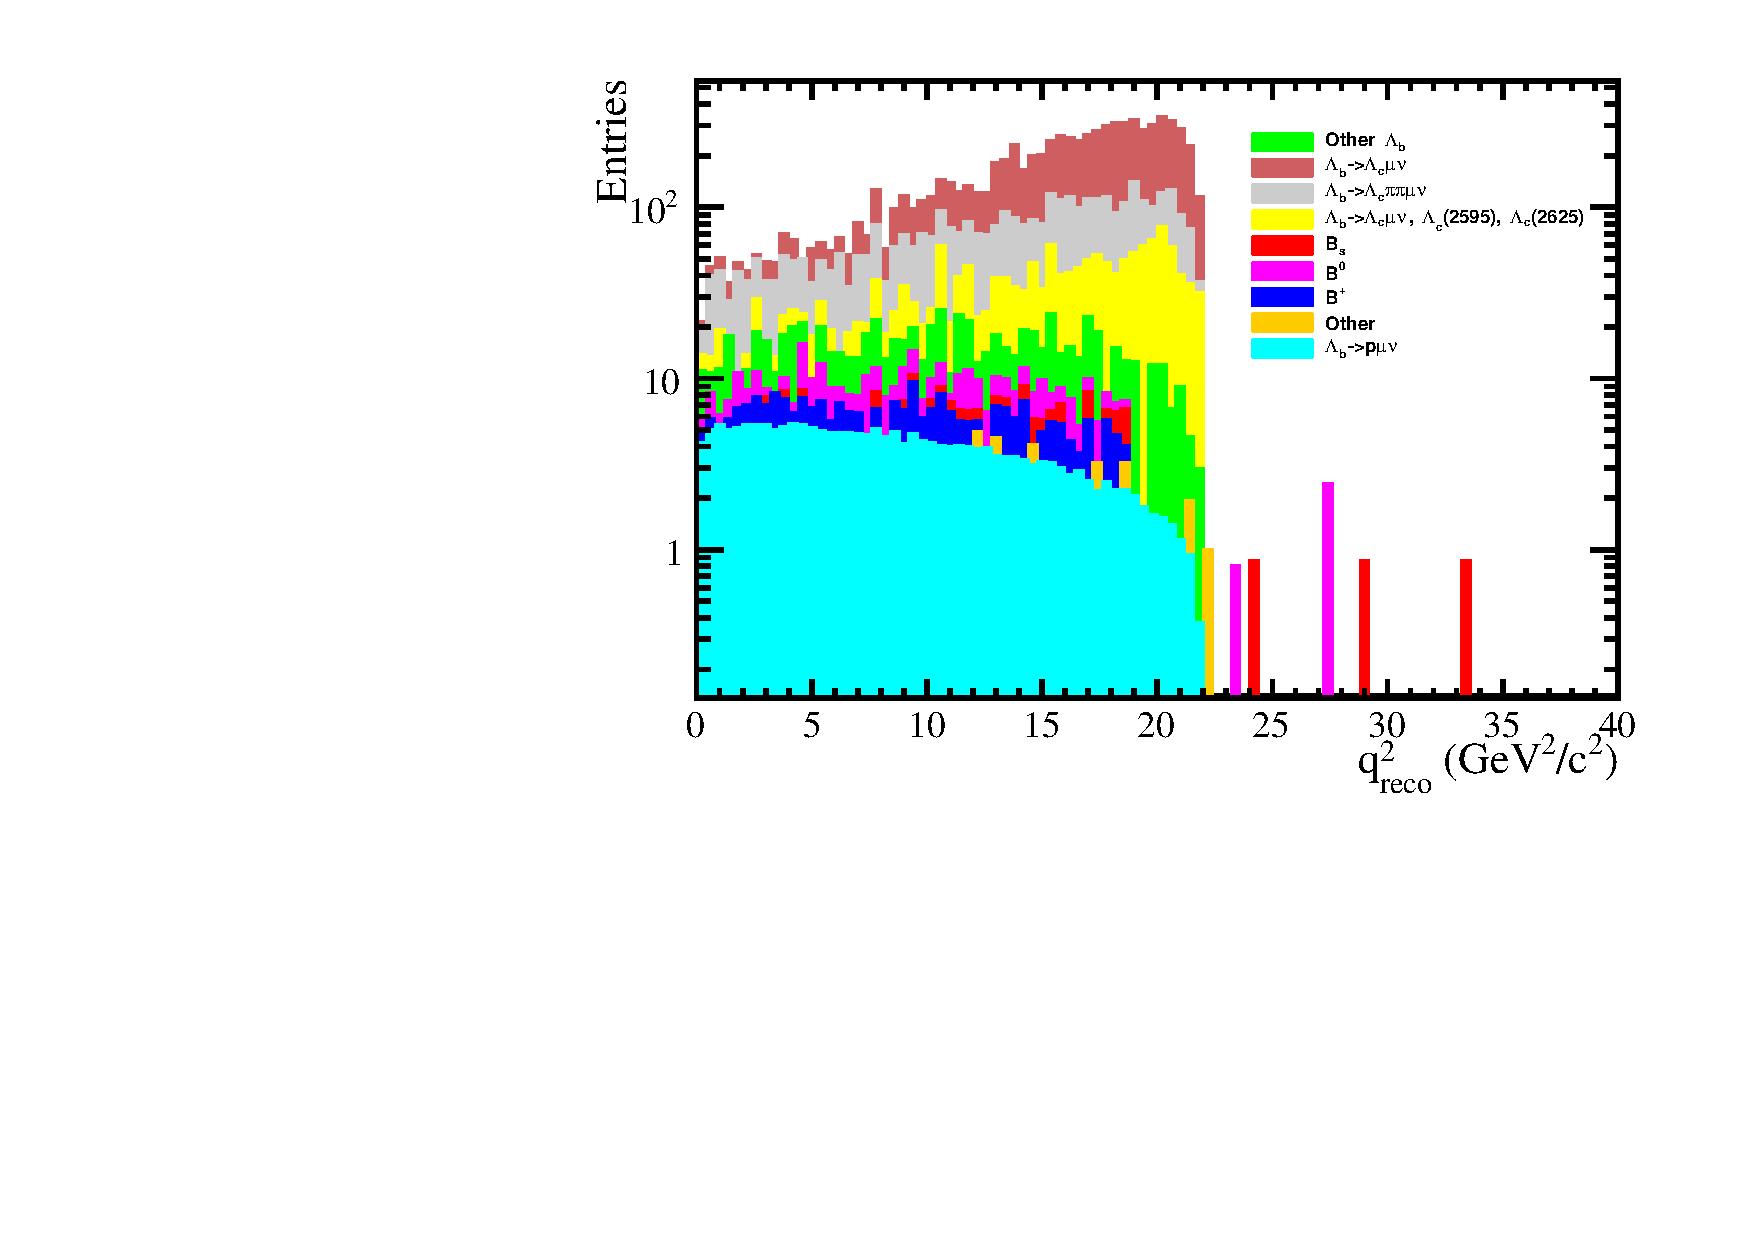
\includegraphics[width=0.45\textwidth]{q2_recon_stacked.pdf} \\
     
       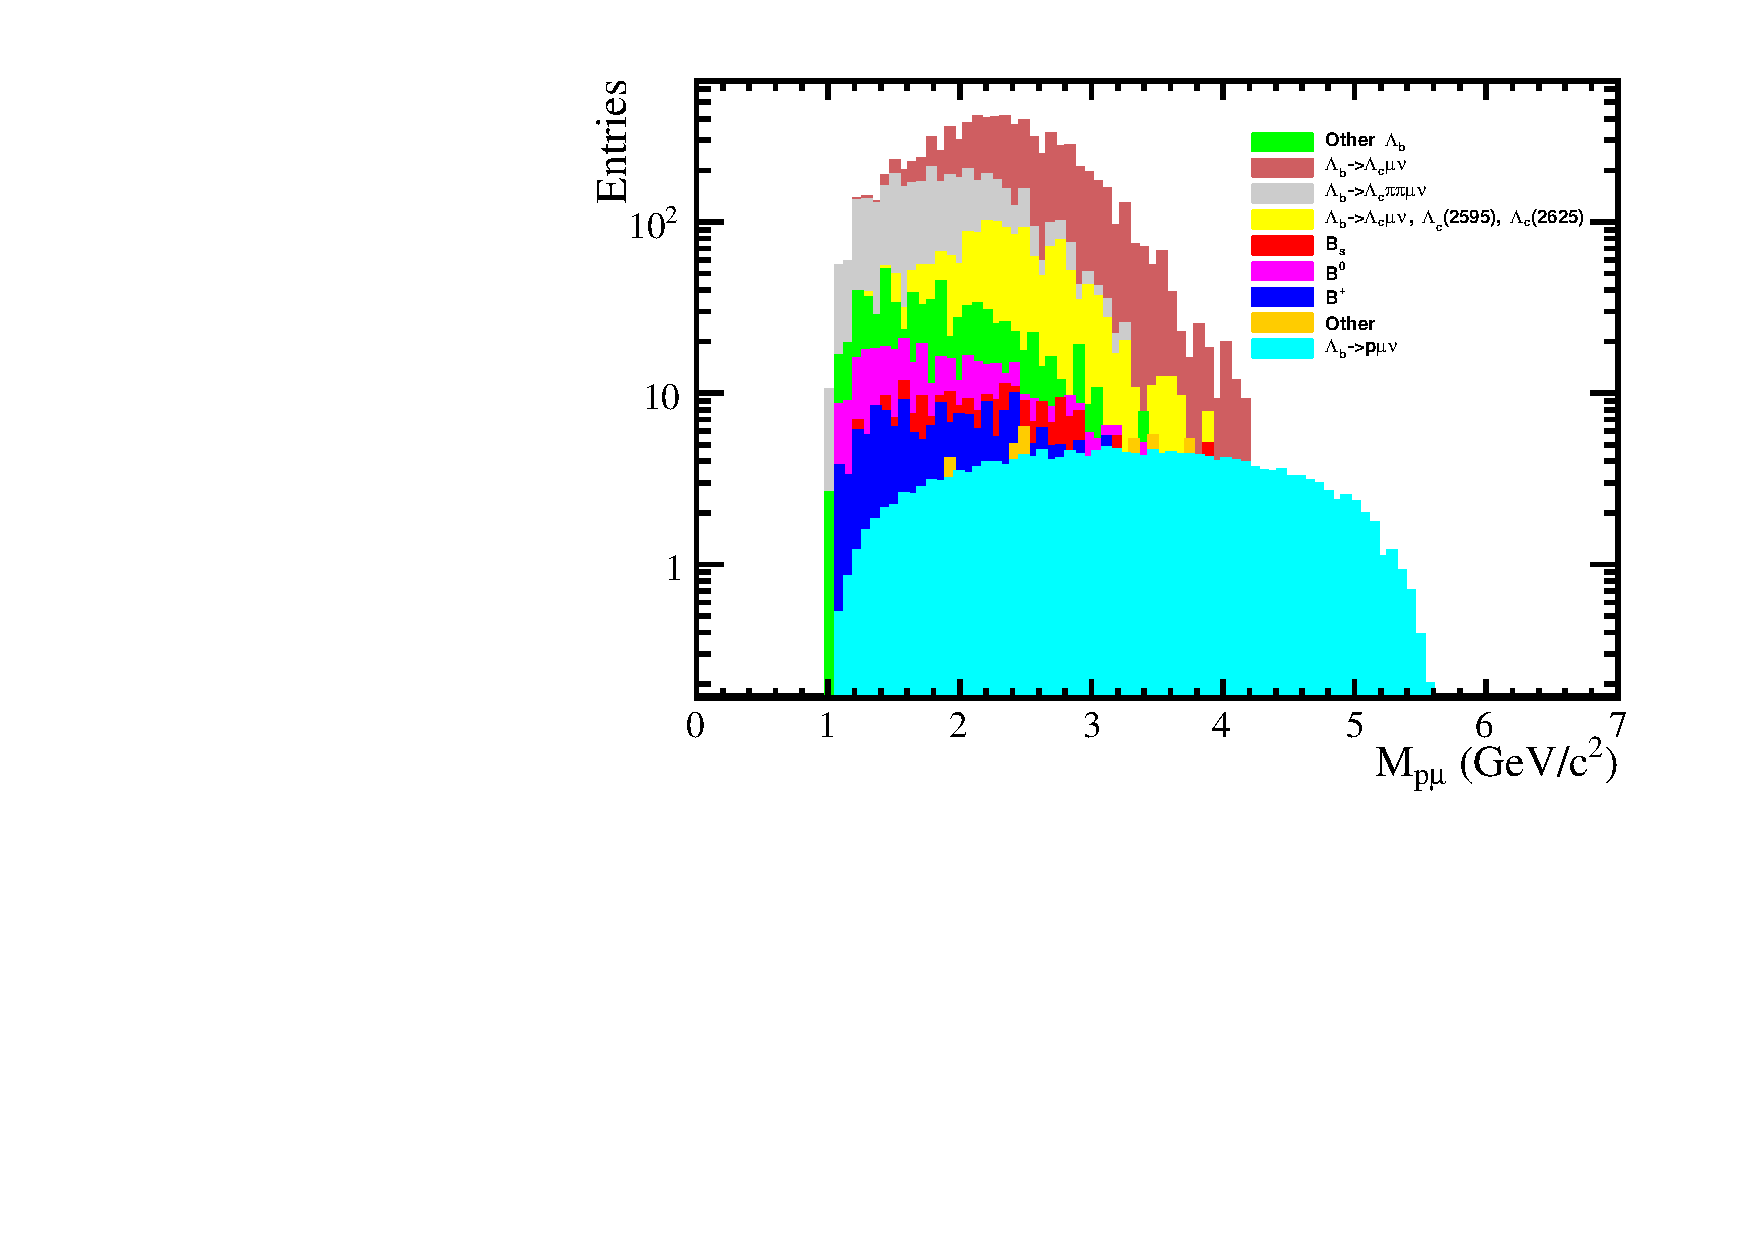
\includegraphics[width=0.45\textwidth]{M_pmu_stacked.pdf}    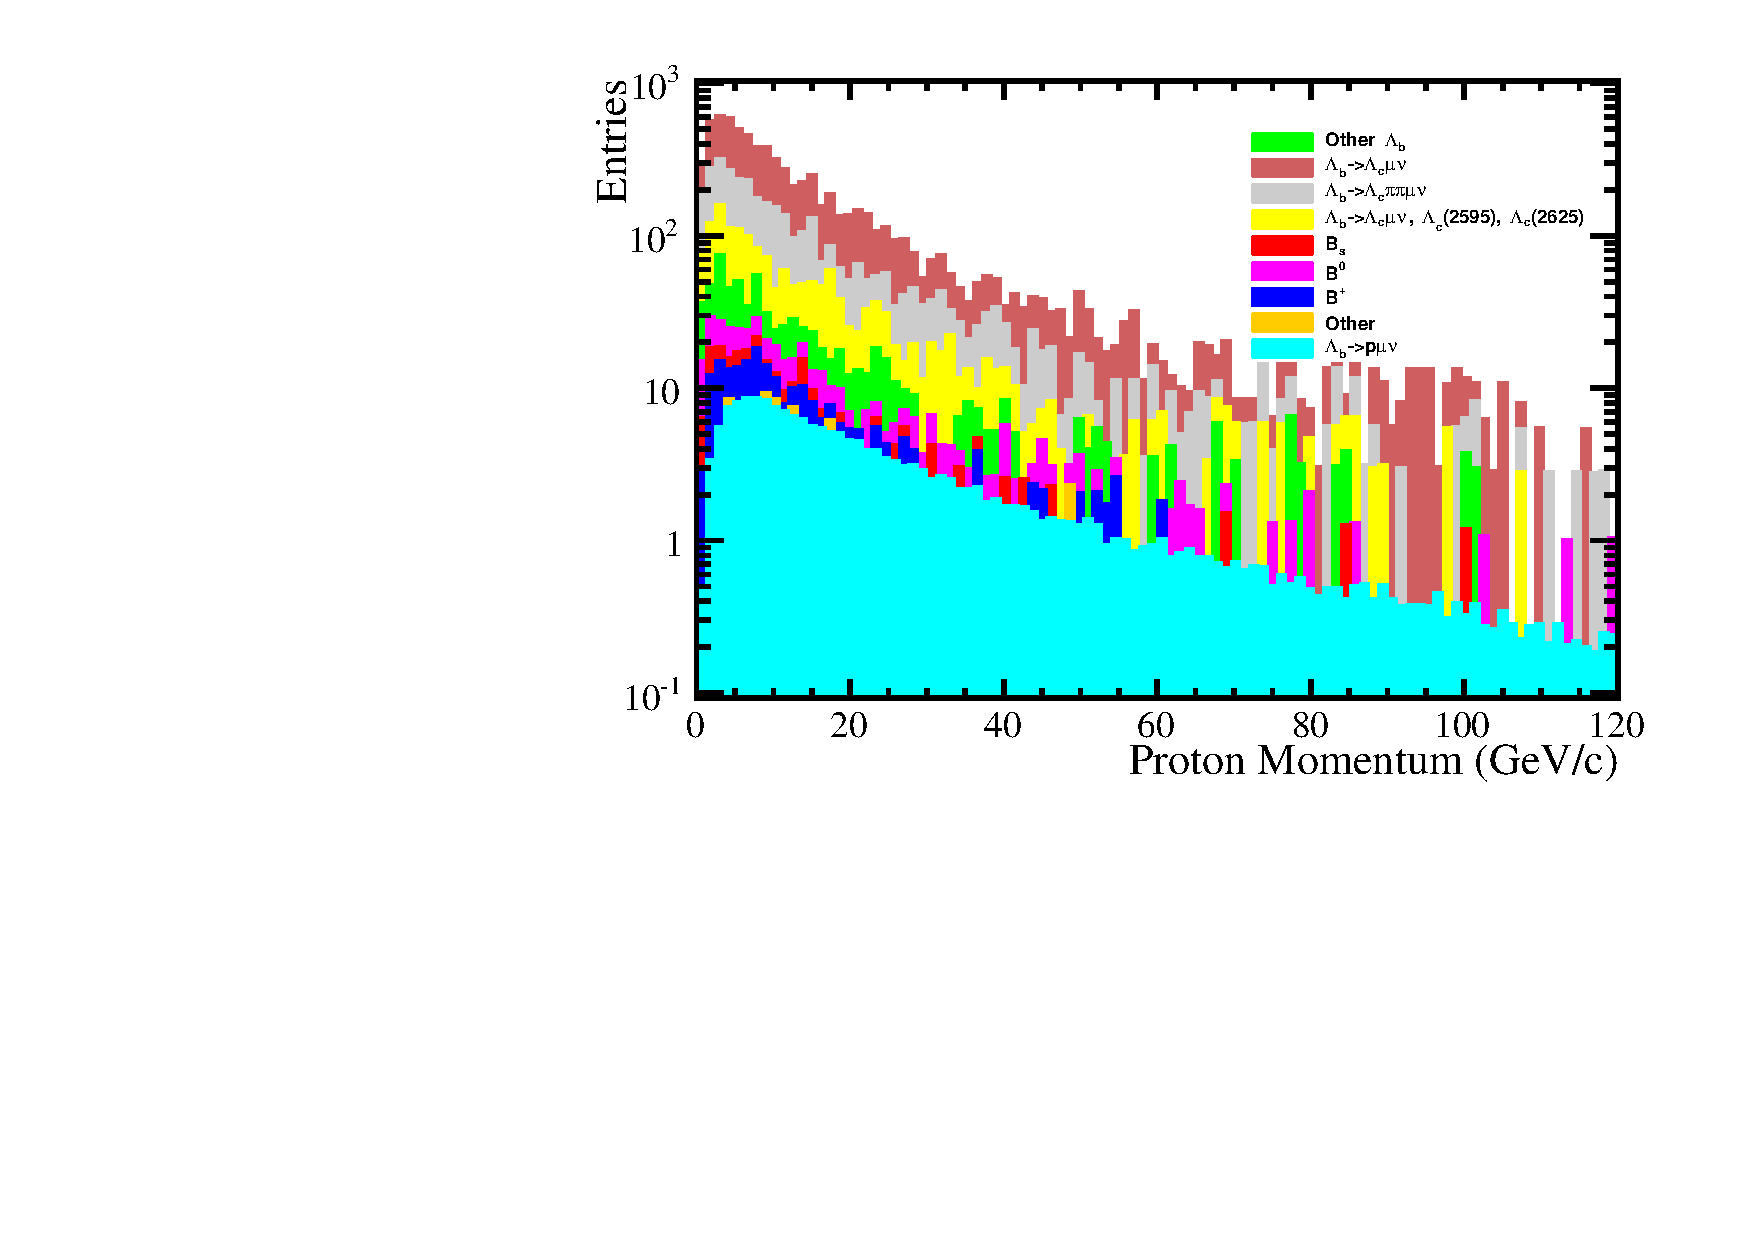
\includegraphics[width=0.45\textwidth]{P_Proton_stacked.pdf} 

}


 
  \frame{
 \frametitle{ Opposite Sign and Same Sign Statistics }
 \begin{itemize}
  \item Find 3391 opposite sign and 716 same sign combinations.
\end{itemize}
\begin{center}
 \hspace{-6cm}  \uline{For Opposite Sign:} \\
 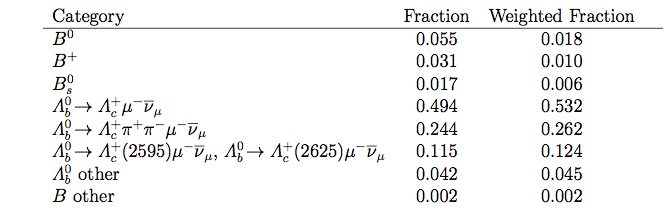
\includegraphics[width=0.75\textwidth]{OS.png}   \\
   \hspace{-6.5cm}  \uline{For Same Sign:} \\
  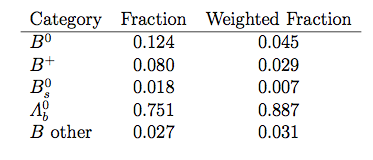
\includegraphics[width=0.4\textwidth]{SS.png}   
  \end{center}
  


}

 \frame{
  \frametitle{Opposite Sign $\pi\mu$ Combinations}
   \begin{itemize}
  \item Can also look for $\pi\mu$ or $K\mu$.
\end{itemize}
      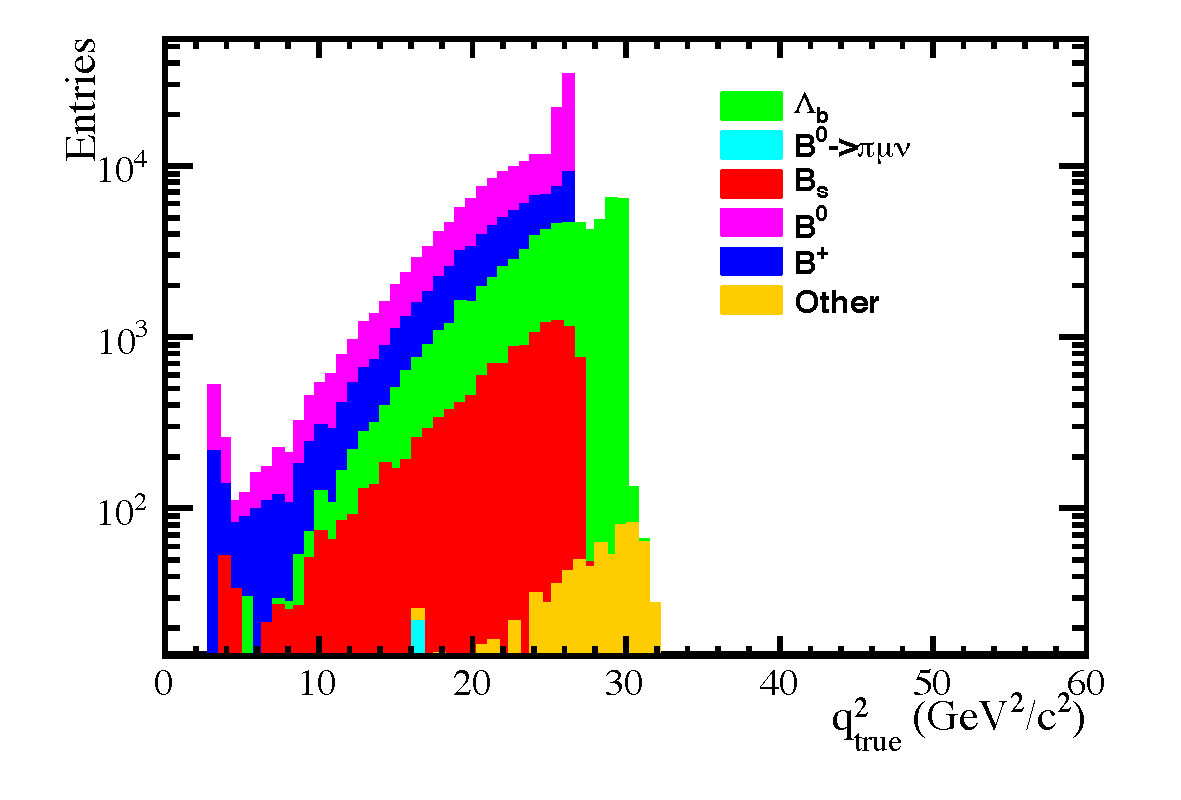
\includegraphics[width=0.4\textwidth]{pimu_q2true_stacked.pdf}    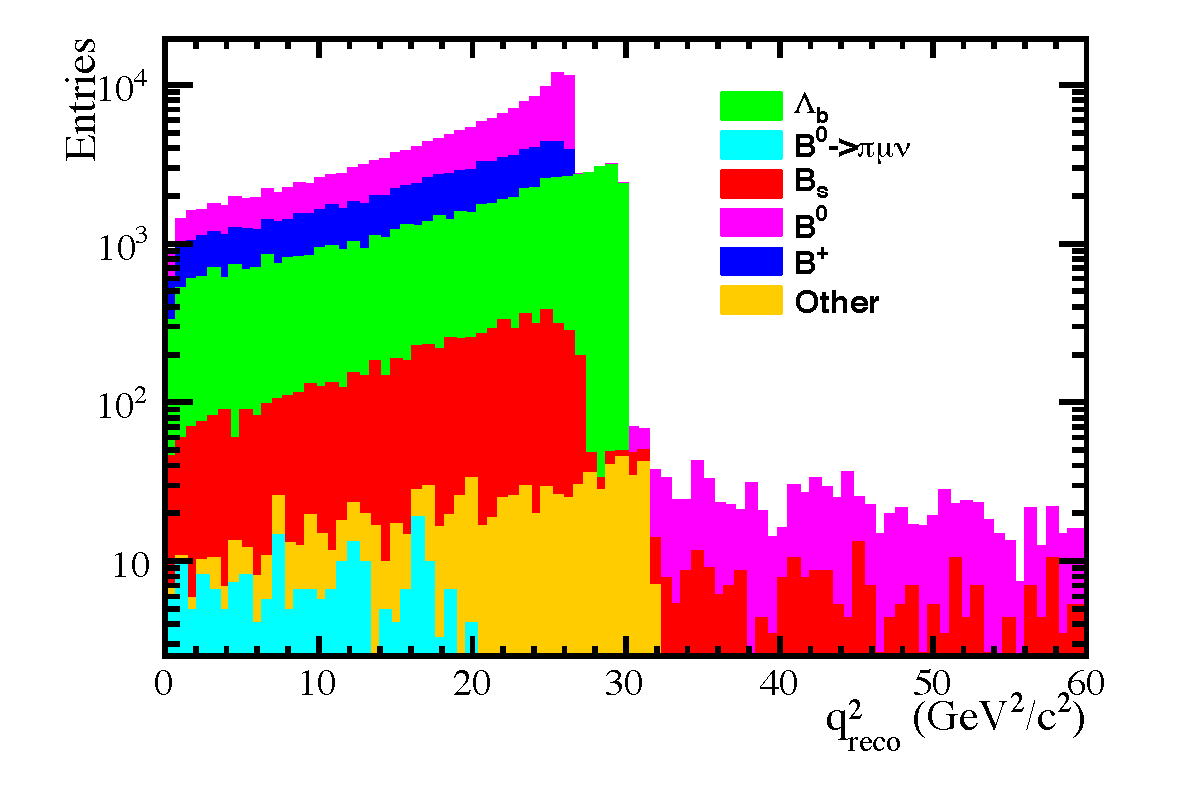
\includegraphics[width=0.4\textwidth]{pimu_q2reco_stacked.pdf} \\
     
       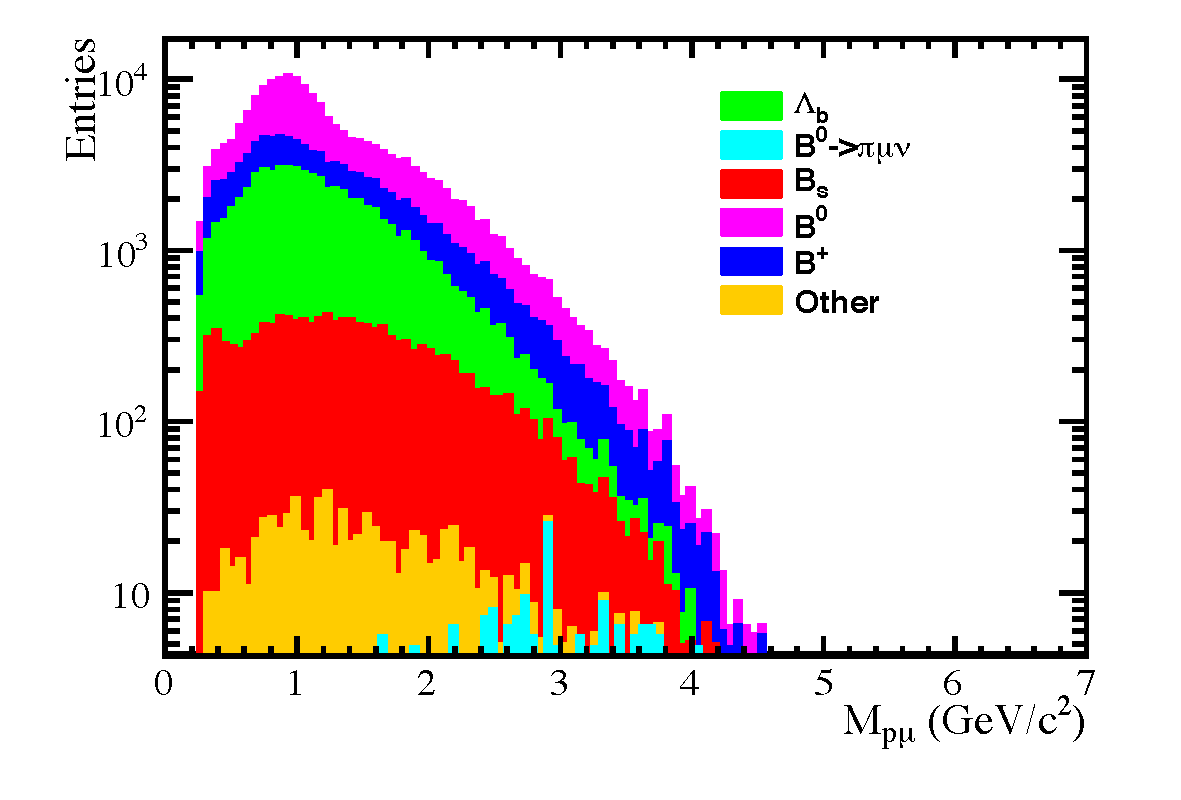
\includegraphics[width=0.4\textwidth]{M_pimu_stacked.pdf}    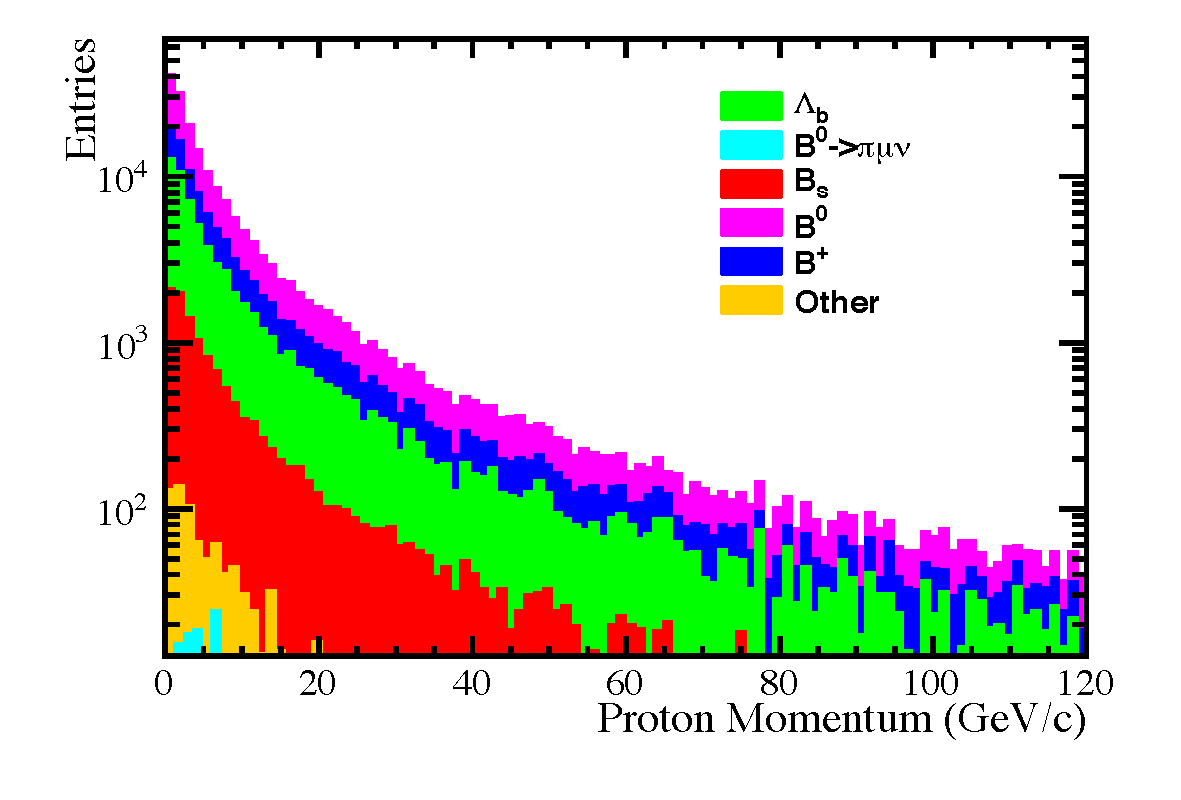
\includegraphics[width=0.4\textwidth]{P_Pion_stacked.pdf} 
}

%%%%%%%%%%%%
\section{Isolation}
 \frame{
 \frametitle{Main backgrounds}
    \begin{itemize}
  \item From generator level studies it is clear that $\Lambda^{0}_{b} \rightarrow \Lambda^{+}_{c} \mu^{-} \overline{\nu}_{\mu}$ is a major background.
  \item This makes sense as branching fraction for $\Lambda^{+}_{c}$ to a proton together with anything  else is $50 \pm 16$\% and $|V_{cb}|^{2}/|V_{ub}|^{2}$$\sim$$100$.
\end{itemize}

\begin{center}
       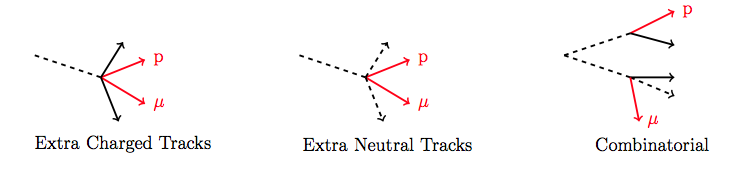
\includegraphics[width=0.9\textwidth]{Isolation1.png}   
       % 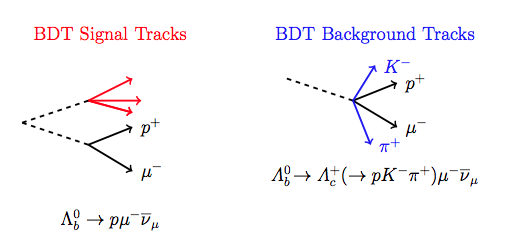
\includegraphics[width=0.45\textwidth]{Isolation2.png} 
       \end{center}

}

  \frame{
 \frametitle{Isolation}
    \begin{itemize}
  \item Train a boosted decision tree to discriminate between charged tracks.
  \item Use following variables: Track $p_{\rm{T}}$, Opening angle, min $\chi^{2}_{IP}$, Ghost Probability,  $\chi^{2}_{IP}$,  Track $\chi^{2}$ and $\chi^{2}_{FD}$.
\end{itemize}
\begin{center}
       %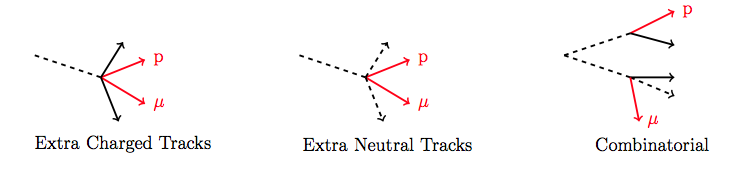
\includegraphics[width=0.9\textwidth]{Isolation1.png}   
        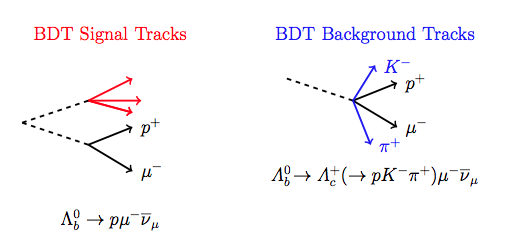
\includegraphics[width=0.8\textwidth]{Isolation2.png} 
       \end{center}
}

  \frame{
 \frametitle{Training Stage}
 
\begin{itemize}
\item Train BDT offline on samples.
  \begin{center}
    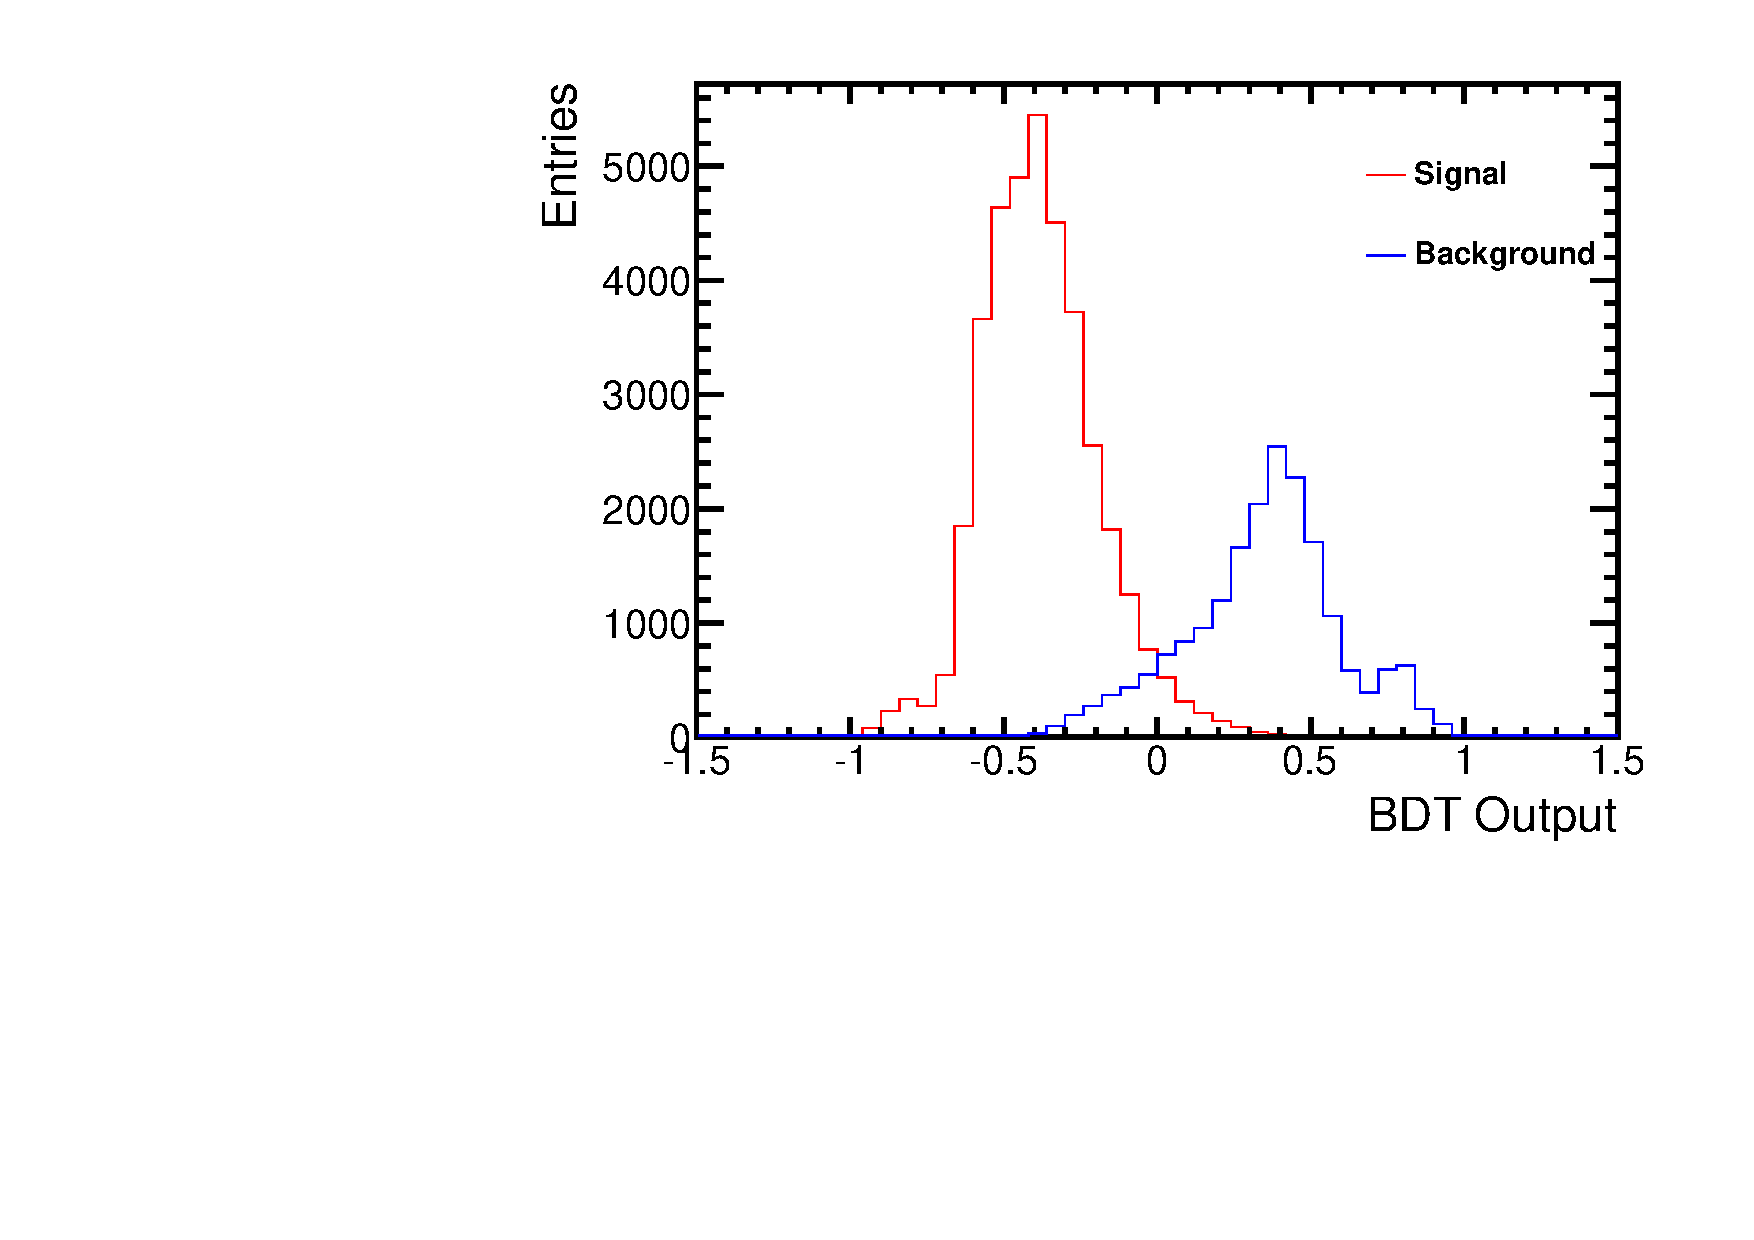
\includegraphics[width=0.8\textwidth]{training.pdf}  
\end{center}

\end{itemize}

}
  \frame{
 \frametitle{Running Stage}
 
\begin{itemize}
\item Run BDT online on all tracks in event. Store maximum BDT output. for each event
  \begin{center}
    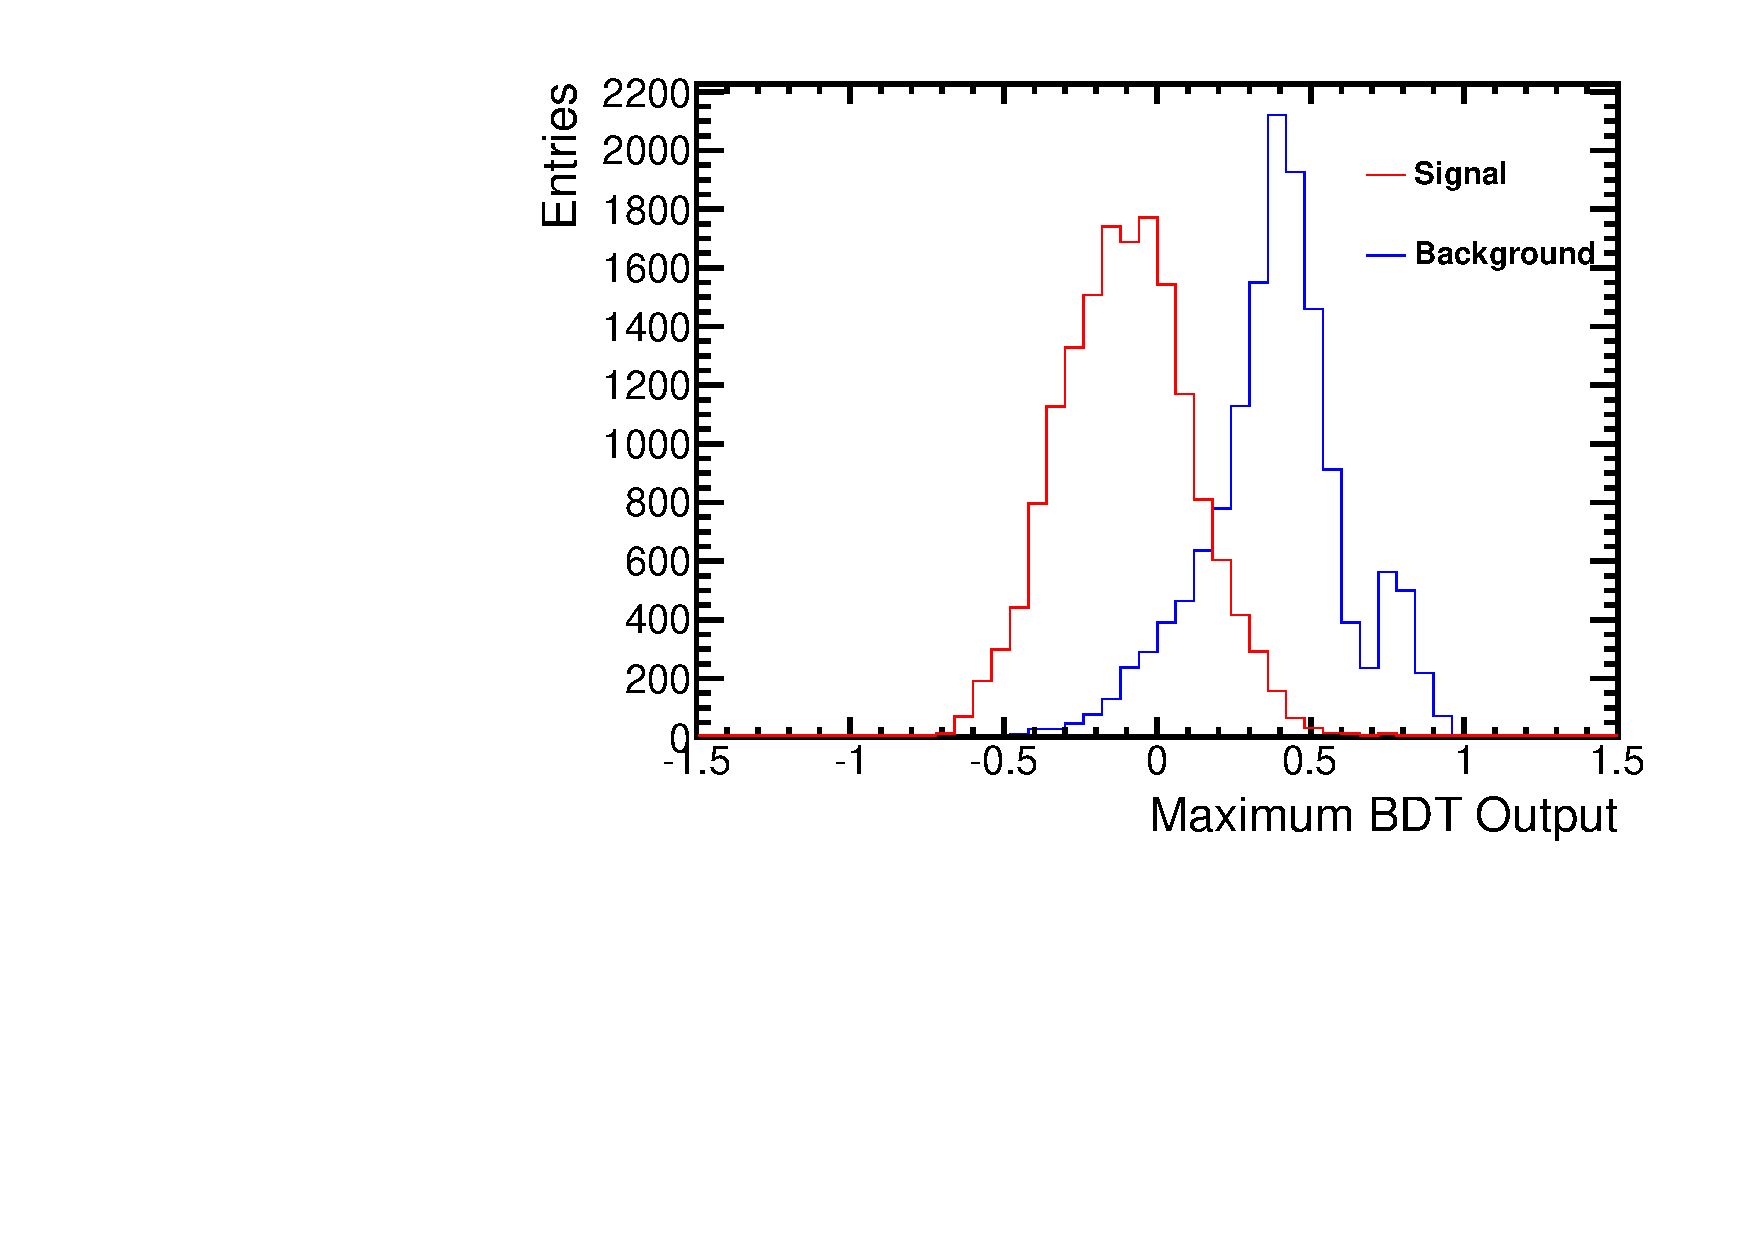
\includegraphics[width=0.7\textwidth]{Isolation_BDT.pdf}  
\end{center}

\end{itemize}

}

\section{$\Lambda_{b} \rightarrow p \mu \nu$ Form Factors}
  \frame{
 \frametitle{$\Lambda_{b} \rightarrow p \mu \nu$ Form Factors}
 The tree-level matrix element for this decay may be written as:
\[
 \mathcal{M} =  -i \frac{G_{F}}{\sqrt{2}} V_{ub} H_{\nu} \overline{u}_{\mu} \gamma^{\nu} (1 - \gamma_{5}) v_{\nu_{\mu}}
\]
 where $H_{\nu} = <N^{+}(p',s')|\overline{u} \gamma_{\nu} (1 - \gamma_{5}) b | \Lambda^{0}_{b}(p,s)>$ 
  \begin{center}
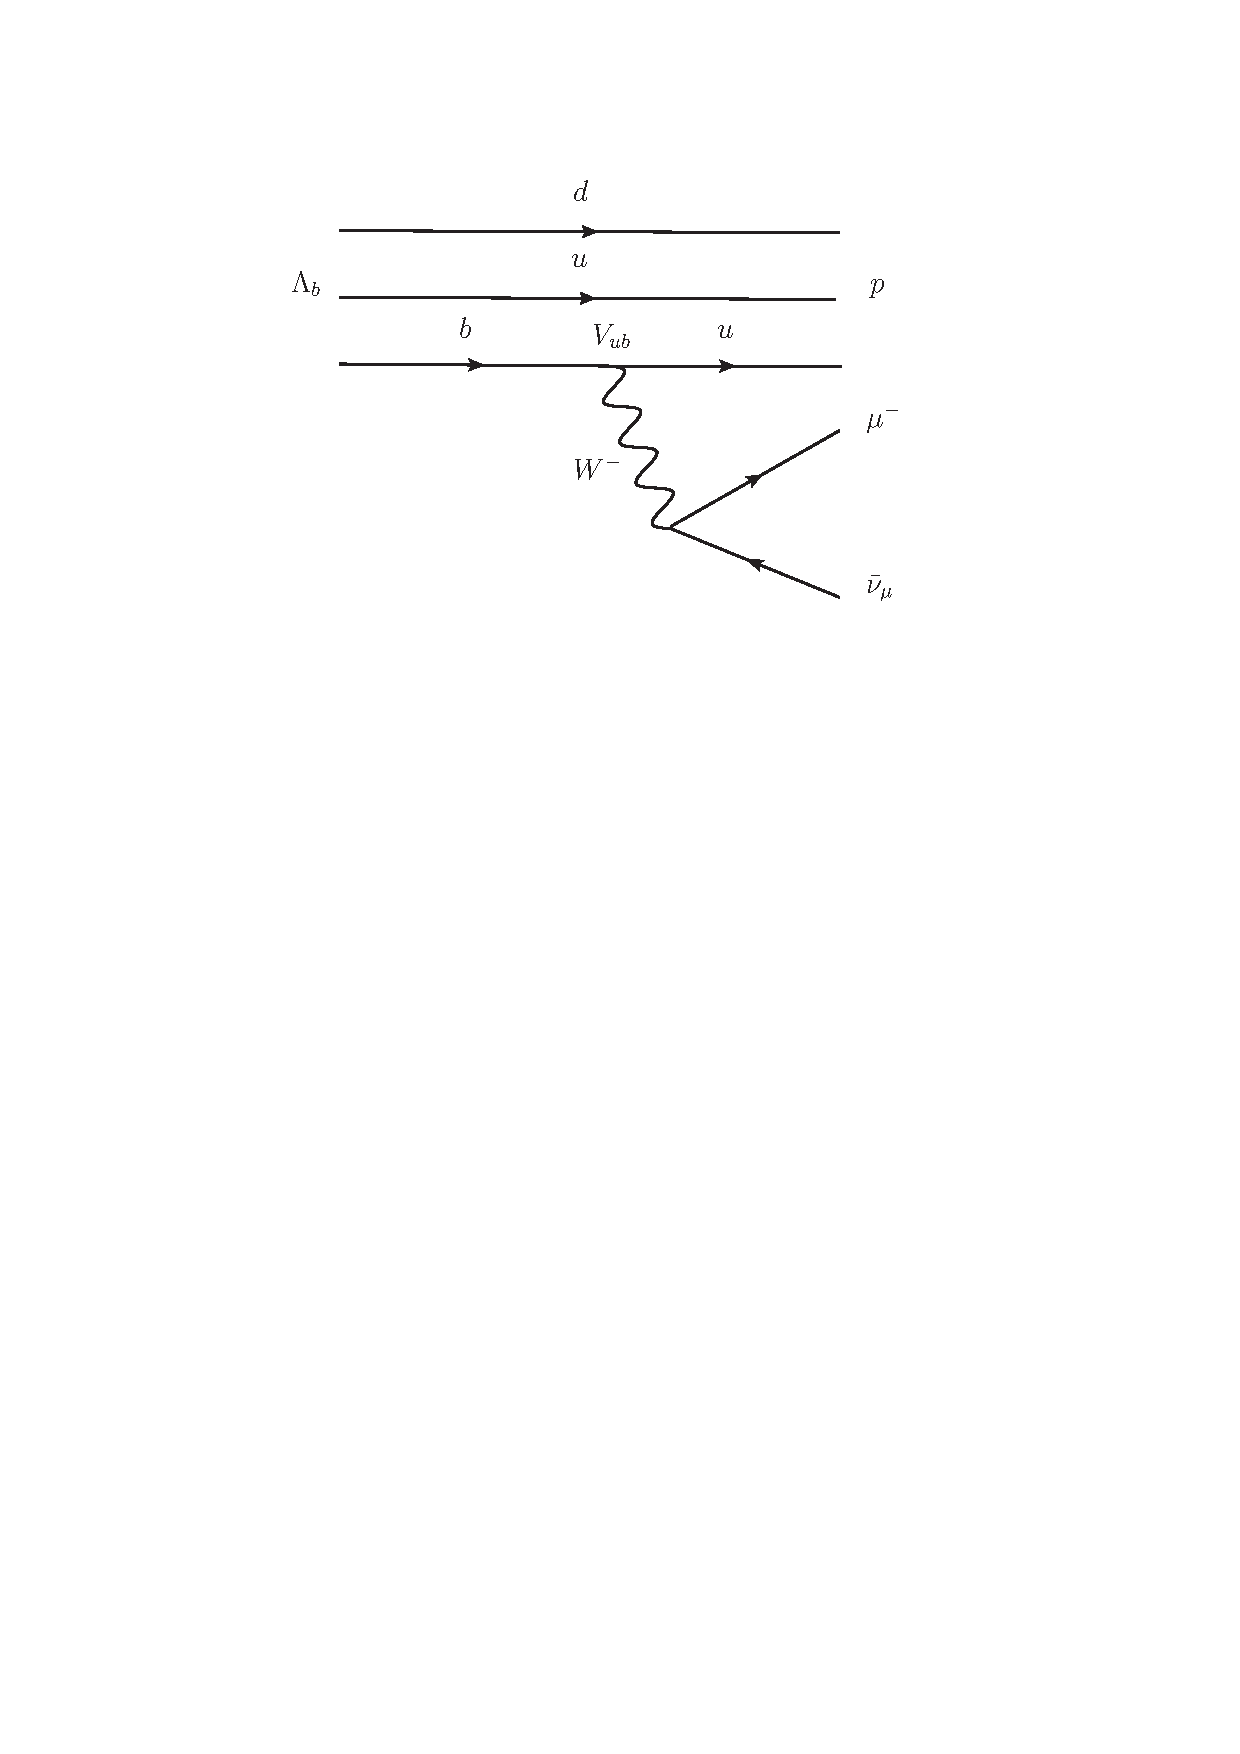
\includegraphics[trim = 15mm 190mm 0mm 30mm, clip, width=8cm]{feynsig.pdf} 
\end{center}

}

  \frame{
 \frametitle{}
\begin{itemize}
\item In general: $H_{\nu} =  \overline{u}_{N}(p') [ F^{V}_{1} \gamma_{\nu} + F^{V}_{2}  v_{\nu} + F^{V}_{3}  v'_{\nu} +  (F^{A}_{1} \gamma_{\nu} + F^{A}_{2}  v_{\nu} + F^{A}_{3}  v'_{\nu}) \gamma_{5}] u_{\Lambda_{b}}(p) $
\item  Light Cone Sum Rules (LCSR) and Lattice QCD can be used to theoretically predict the 6 form factors.
\end{itemize}
 \hspace{0.5cm}  \uline{LCSR, arXiv:1108.2971}  \hspace{1cm} \uline{LQCD, arXiv:1306.0446}\\
  \hspace{0.5cm}  \uline{A. Khodjamirian et al.}  \hspace{1cm} \uline{W. Detmold et al.}
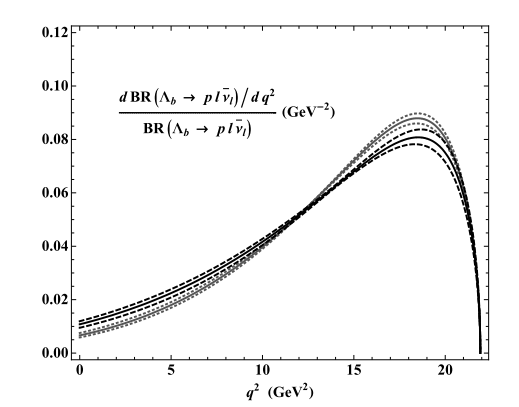
\includegraphics[width=0.45\textwidth]{LCSR.png} 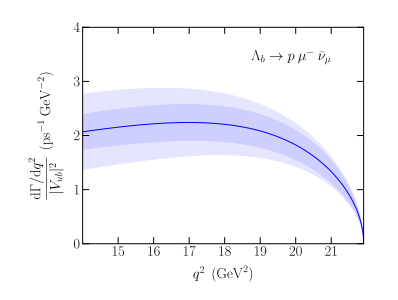
\includegraphics[width=0.5\textwidth]{LQCD.png} 

}

  \frame{
 \frametitle{}
\begin{itemize}
\footnotesize
\item  Theoretical predictions give a very different prediction for the $q^{2}$ dependence of the differential rate, $\frac{d\Gamma}{dq^{2}}$ to the prediction purely based on phase space.
\item Create a class in EvtGen to compute the form factors for a given value of $q^{2}$.
\item Use LCSR predictions provided by arXiv:1108.2971:
\item Strong rise at high $q^{2}$ compared to $B\rightarrow \pi \mu \nu$ as for $\Lambda_{b} \rightarrow p \mu \nu$ width contains only a S-wave phase-space factor (arXiv:1108.2971).
\end{itemize}
\begin{center}
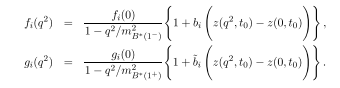
\includegraphics[width=0.5\textwidth]{param.png}  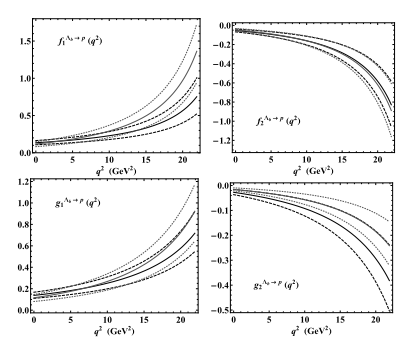
\includegraphics[width=0.4\textwidth]{FF.png} 
\end{center}
}

  \frame{
 \frametitle{LCSR and Phase-space generator level MC}
      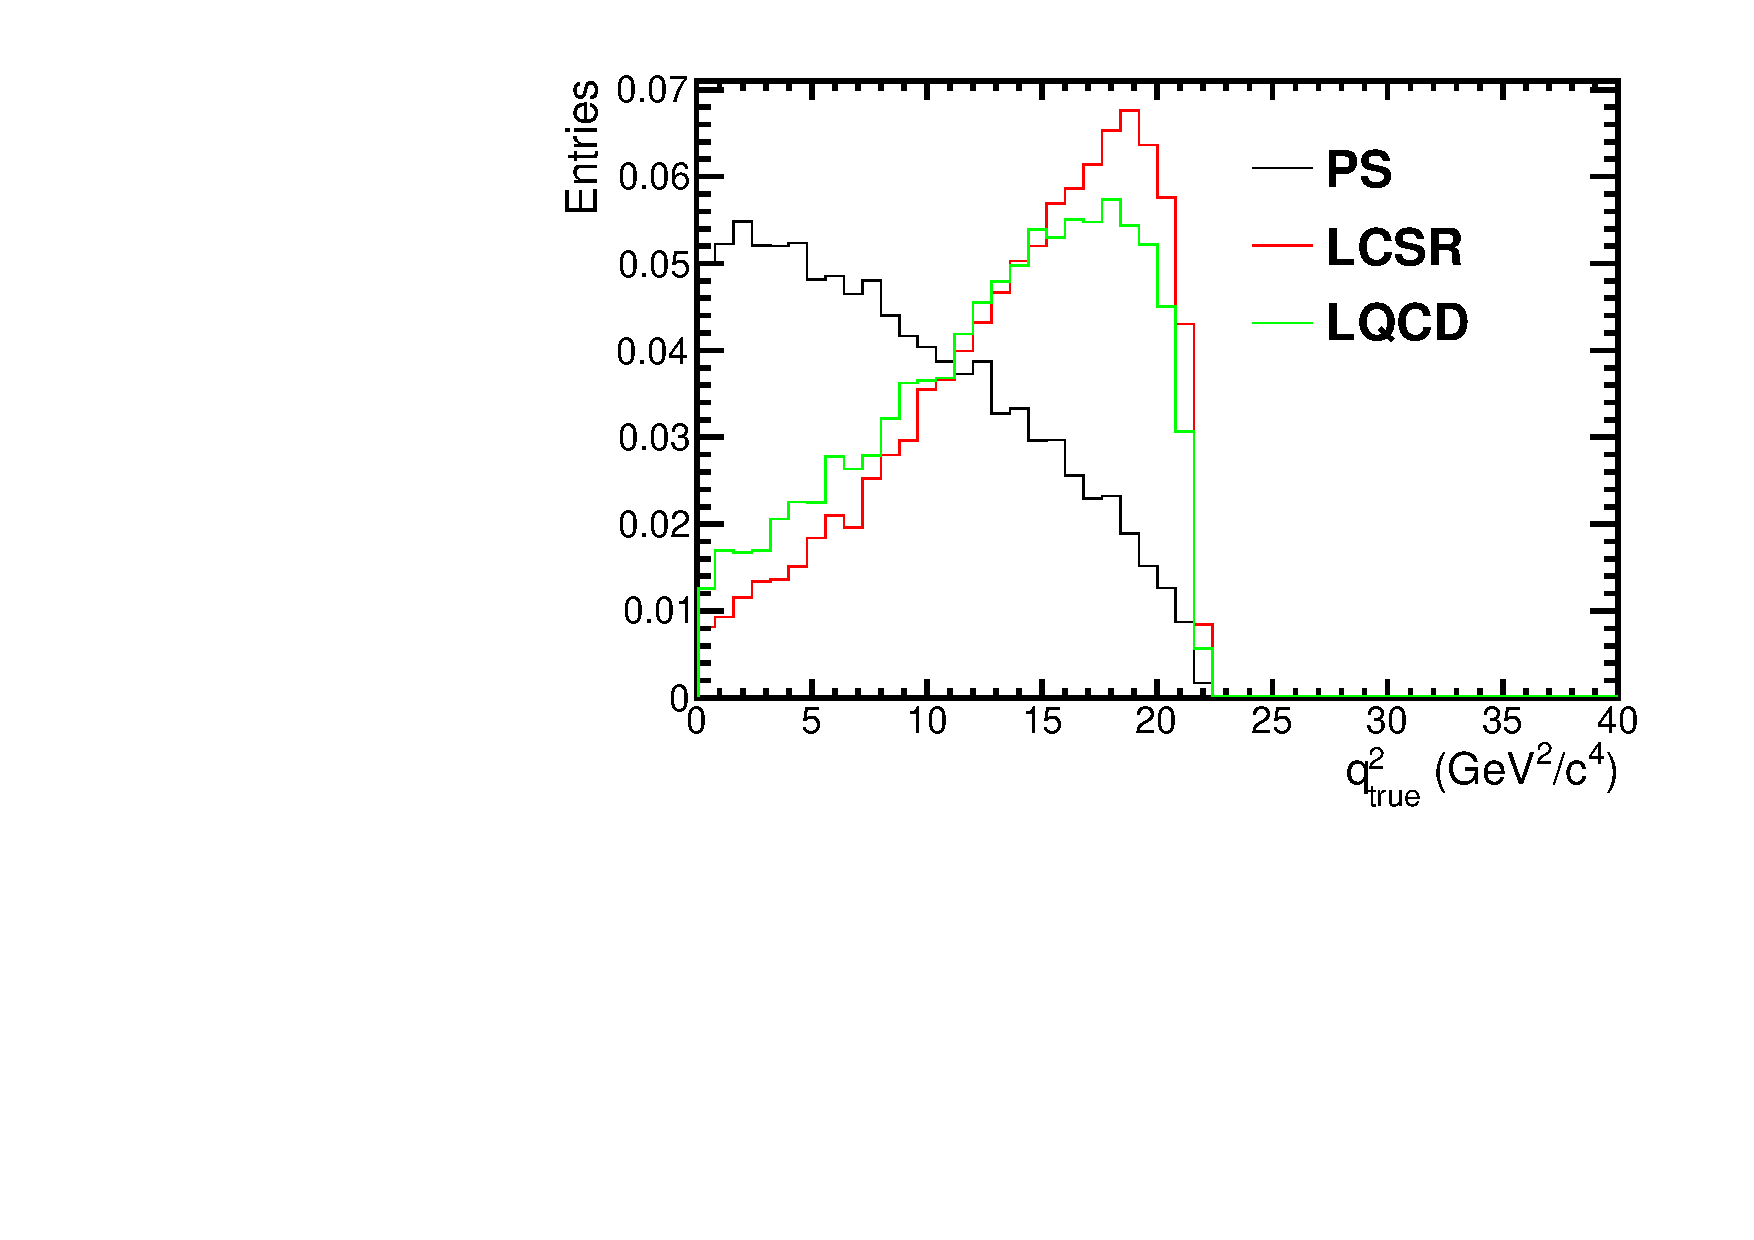
\includegraphics[width=0.4\textwidth]{PSpace_q2vsX/q2_trueSIG.pdf}    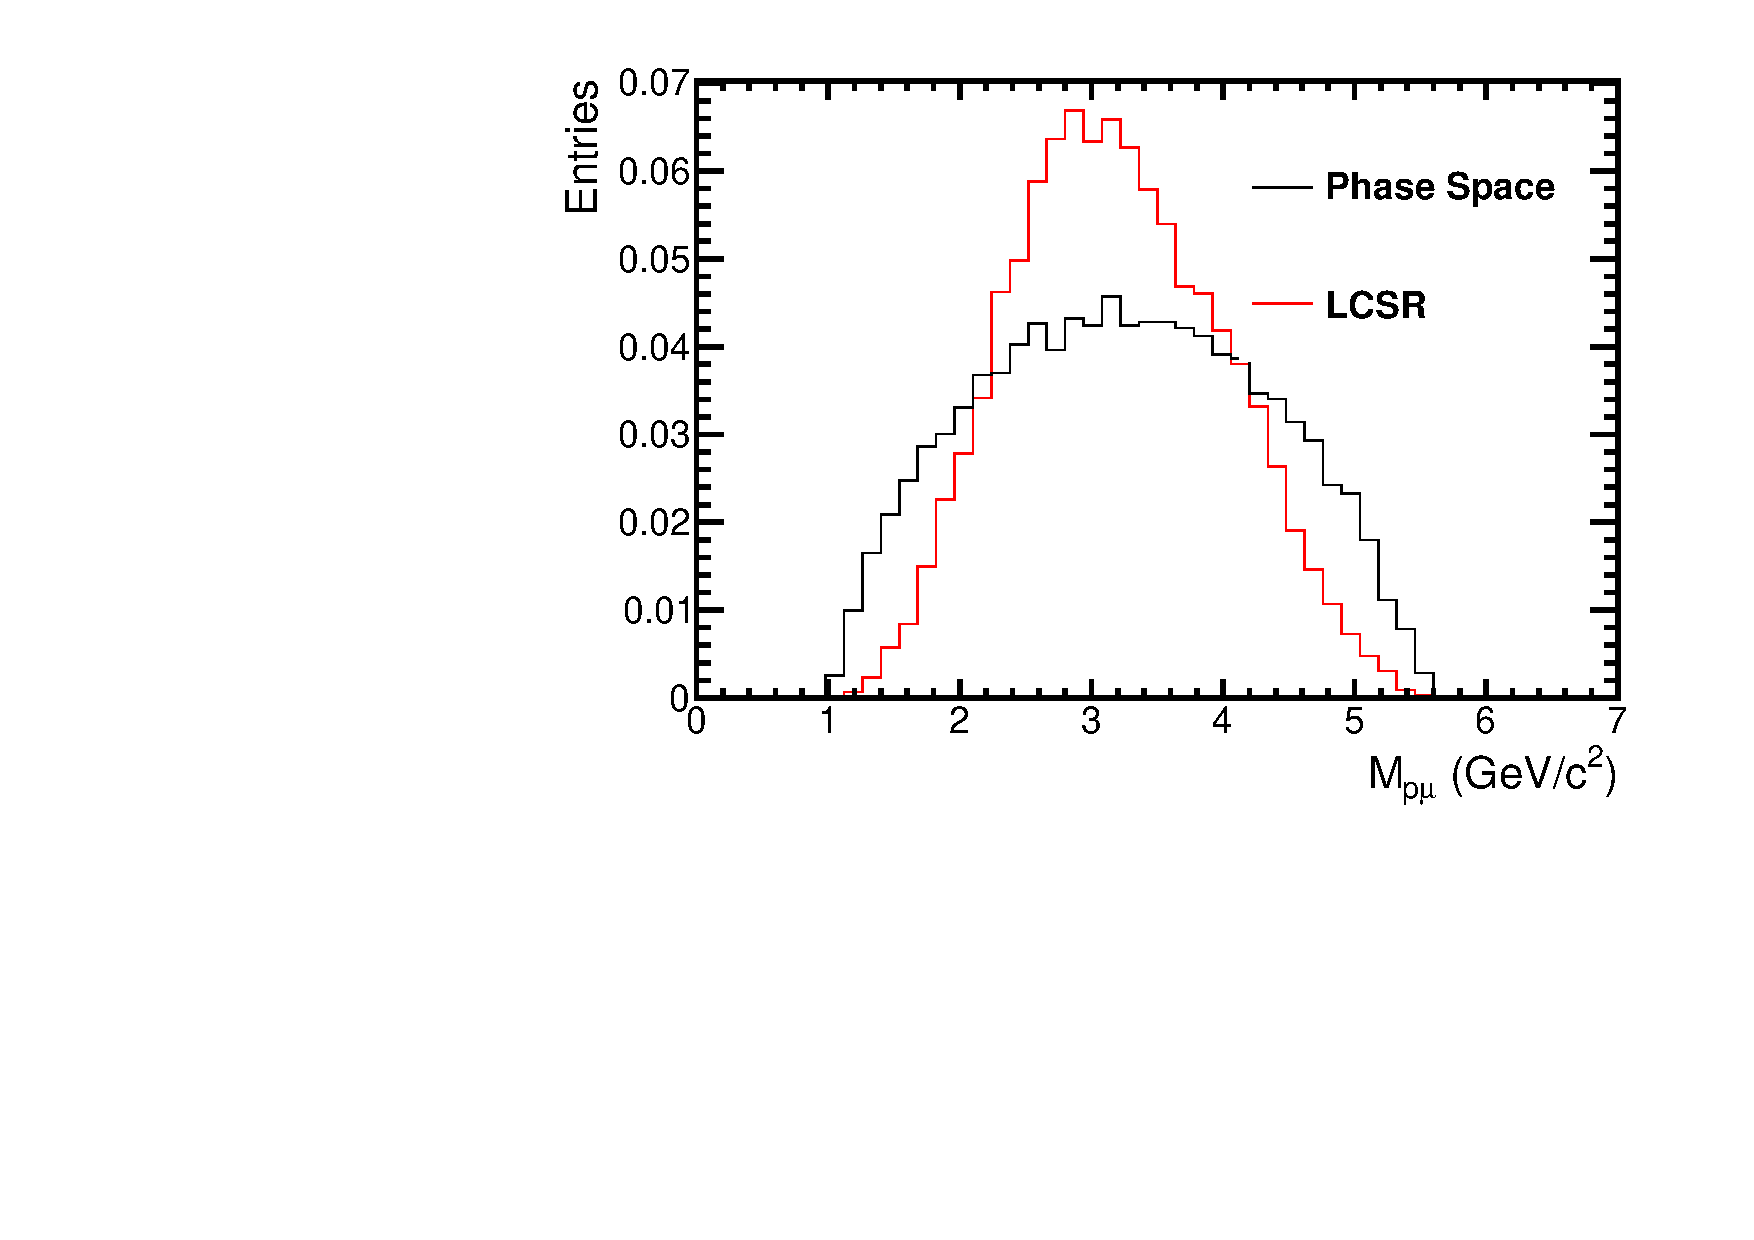
\includegraphics[width=0.4\textwidth]{M_pmuSIG.pdf} \\
     
       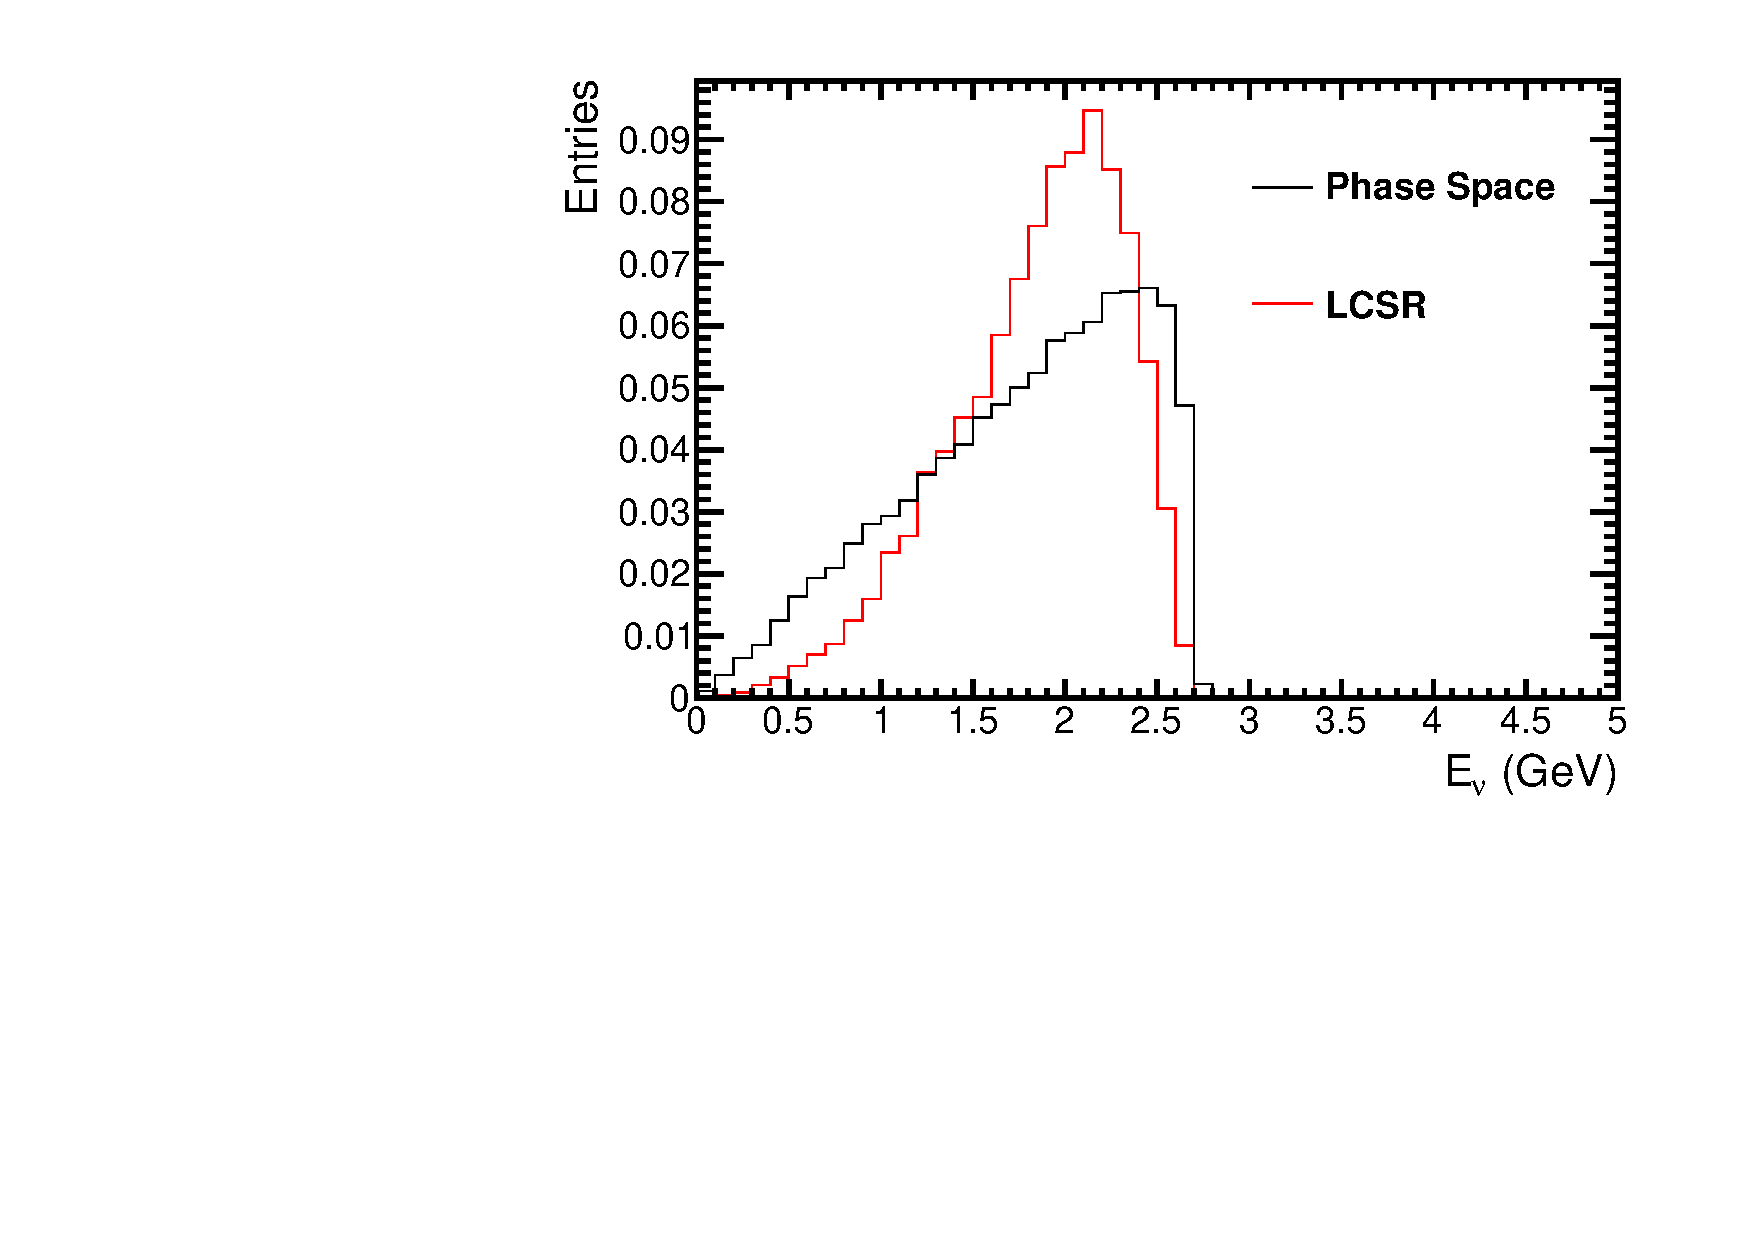
\includegraphics[width=0.4\textwidth]{E_nuSIG.pdf}    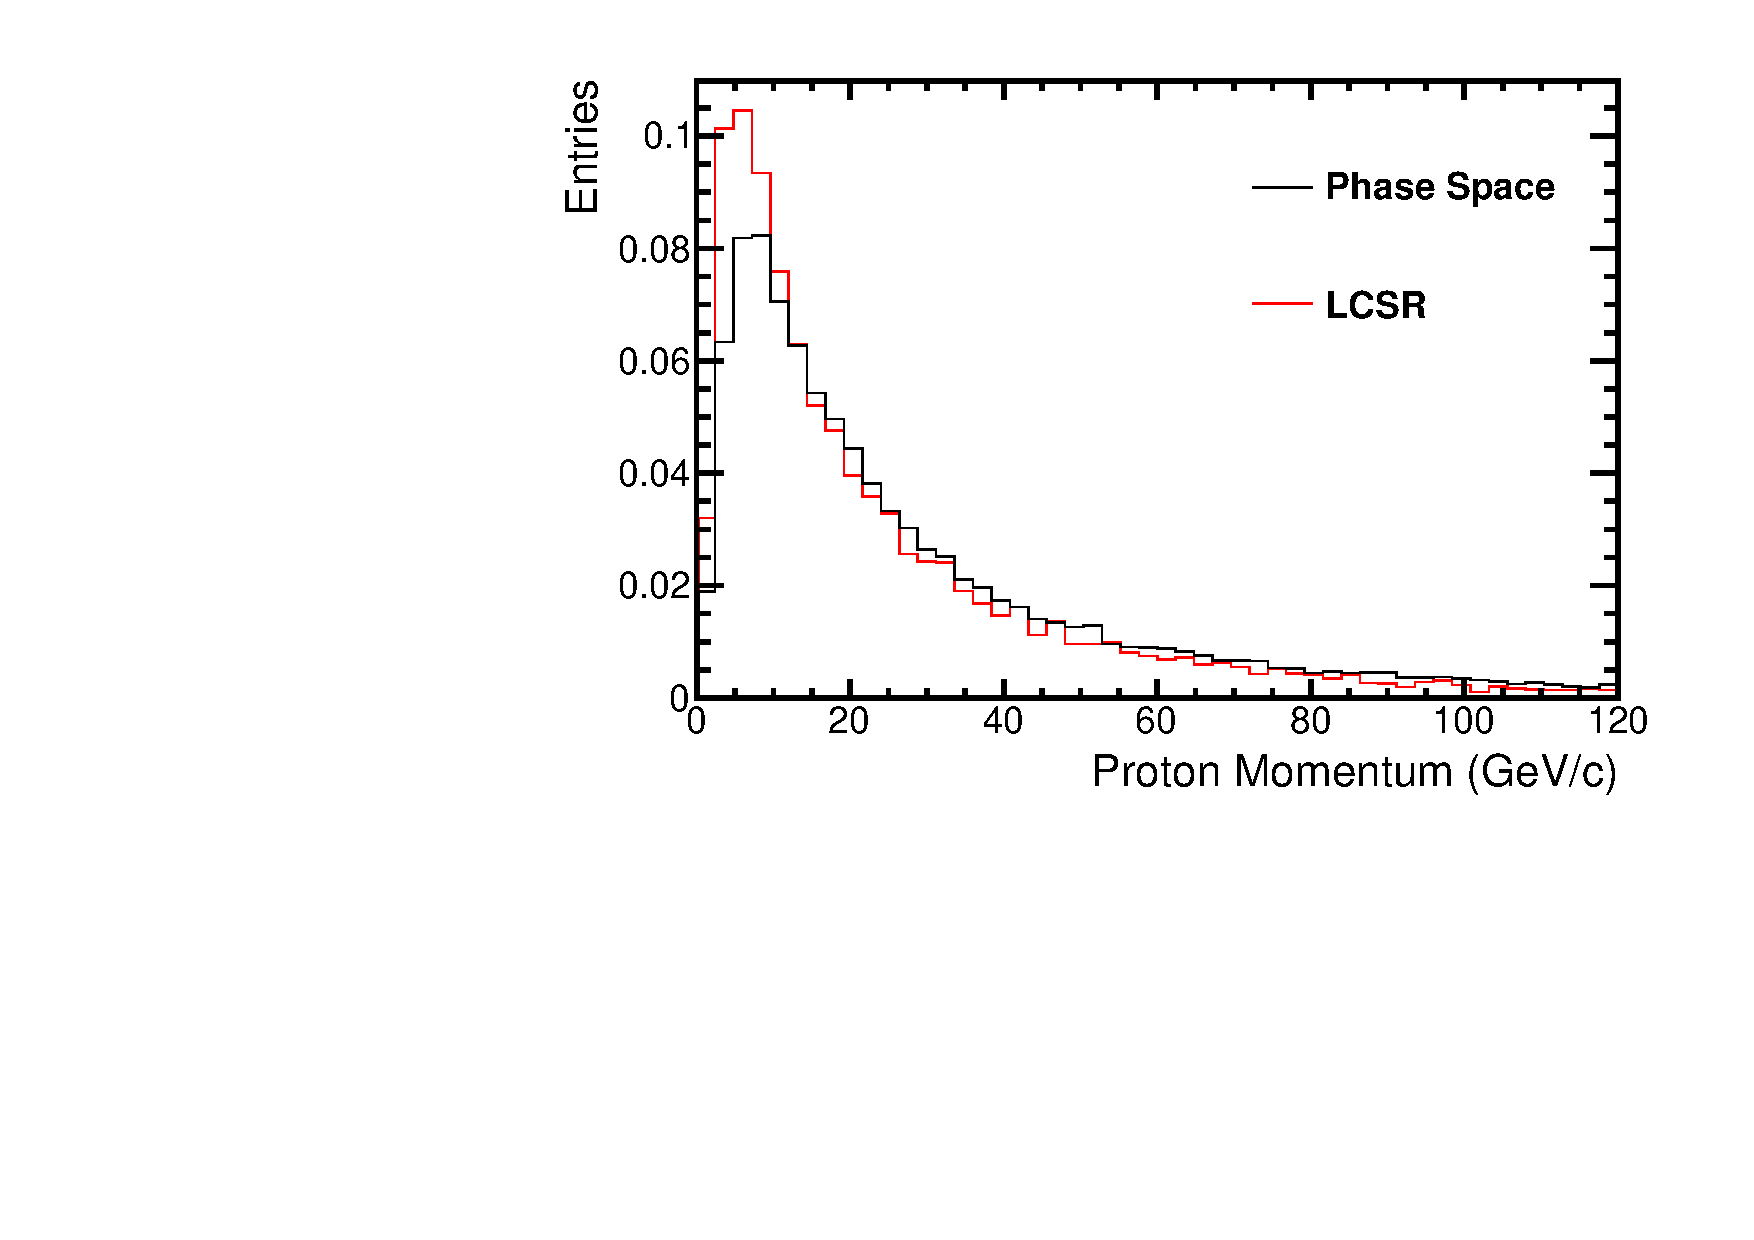
\includegraphics[width=0.4\textwidth]{P_ProtonSIG.pdf} 
}

  \frame{
 \frametitle{}
  \hspace{2cm}  \uline{LCSR}  \hspace{4cm} \uline{Phase Space}
      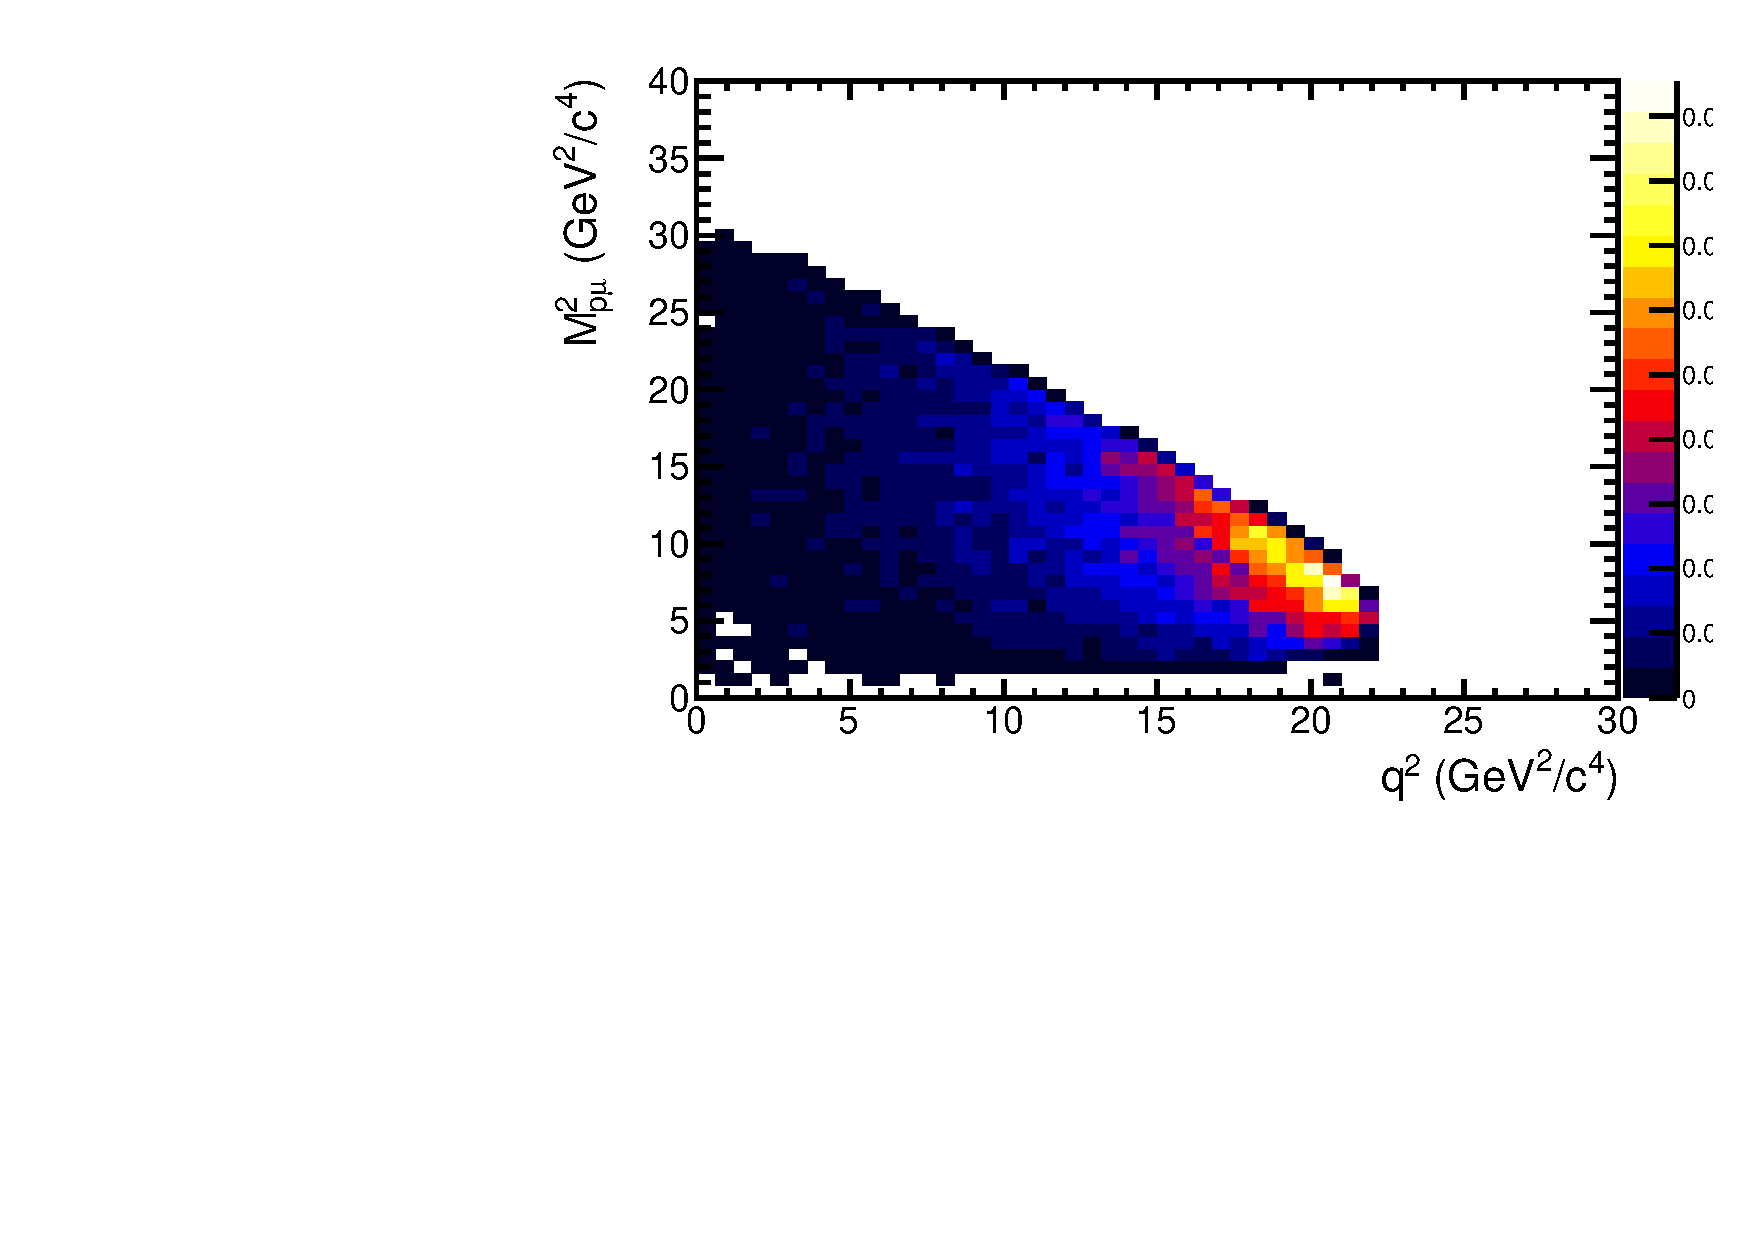
\includegraphics[width=0.5\textwidth]{LCSR_q2vsX/M_pmu.pdf}    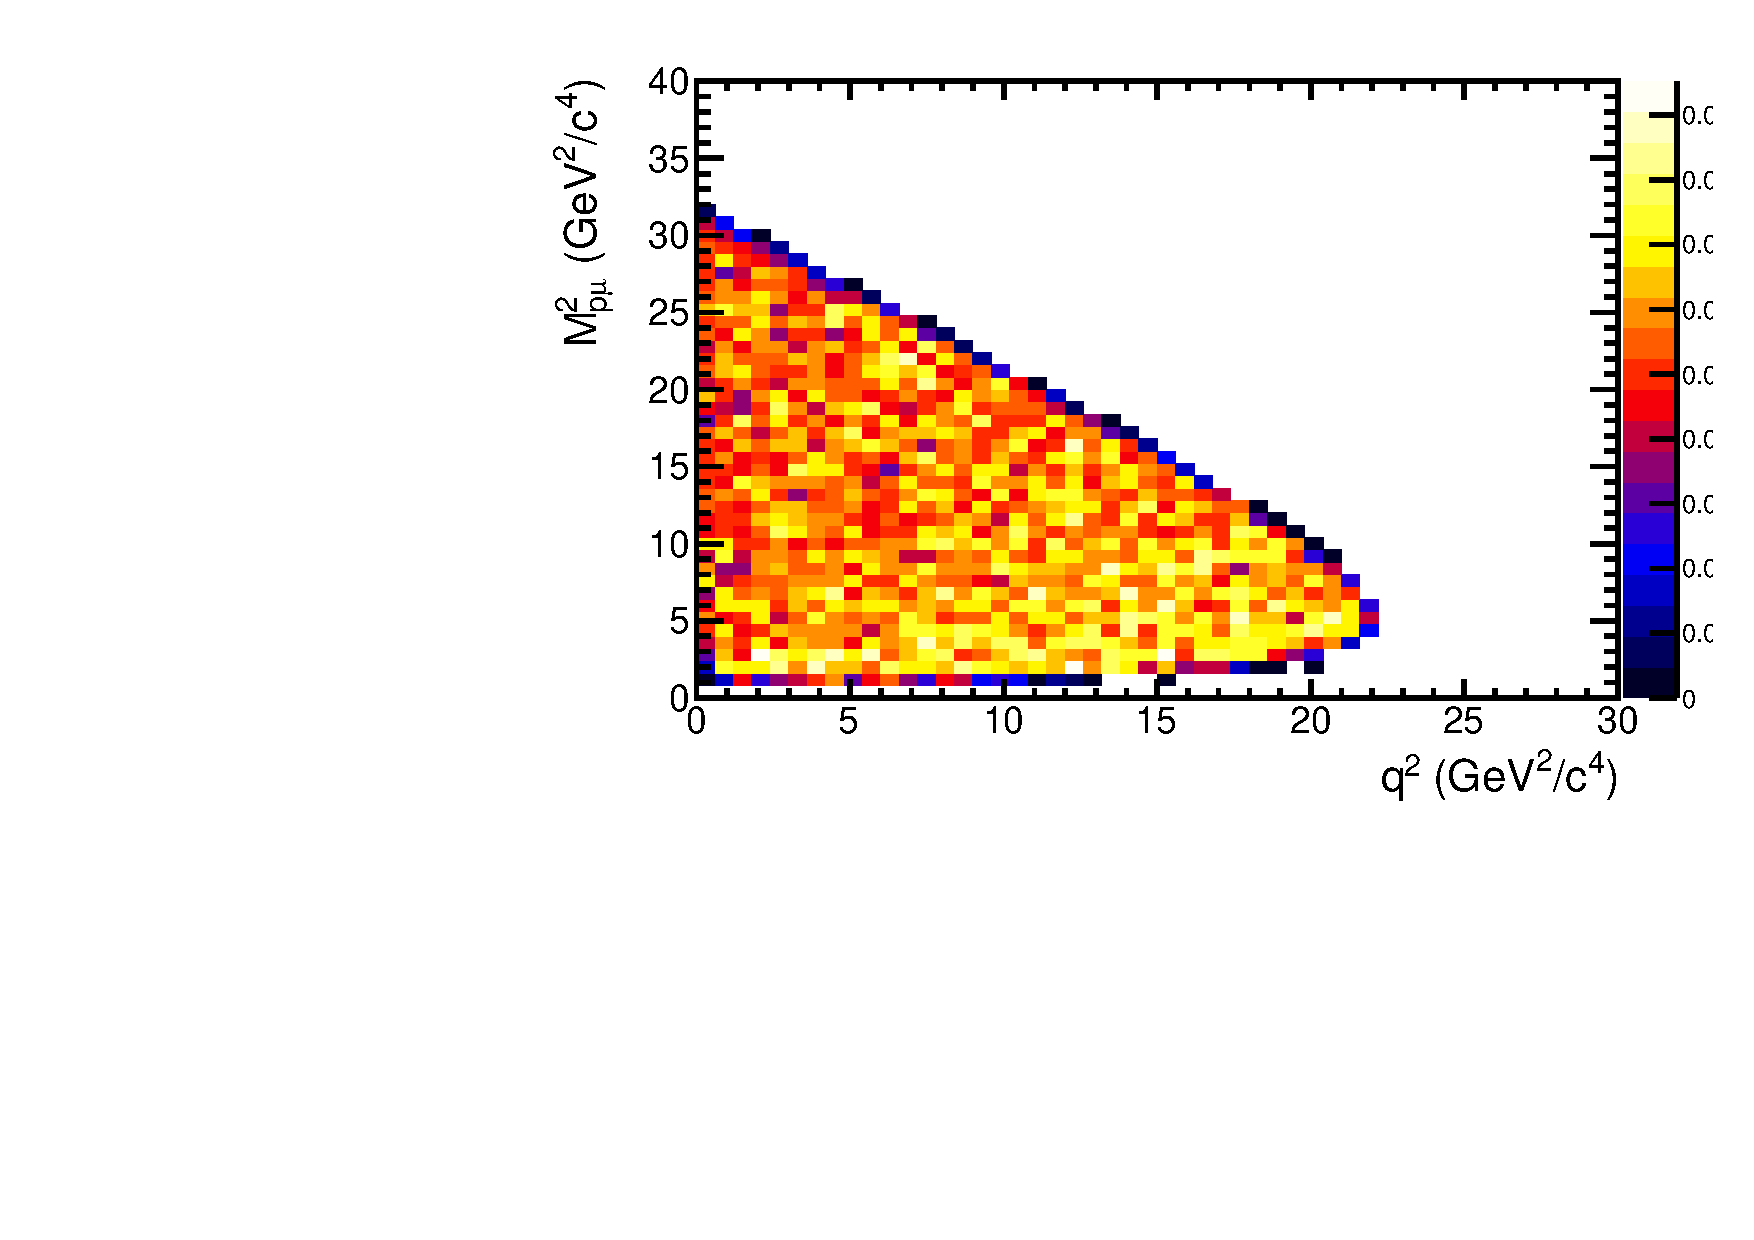
\includegraphics[width=0.5\textwidth]{PSpace_q2vsX/M_pmu.pdf} \\
     
    
}


%%%%new section
\section{Conclusion}



  \frame{
 \frametitle{Conclusion}
 \begin{itemize}
  \setlength{\itemsep}{5pt}
   \item Generator level studies indicate that the decay $\Lambda^{0}_{b} \rightarrow \Lambda^{+}_{c} \mu^{-} \overline{\nu}_{\mu}$ and related decay modes will form a major background to this decay.
    \item Isolation can help reduce backgrounds involving additional charged tracks.  Still need to optimise this.
    \item New MC required which makes use of form factor predictions for $\Lambda_{b} \rightarrow p \mu \nu$.
   \item Methods for estimating or rejecting the combinatorial background required.
   \end{itemize}

}

}
 \end{document}